% UCL Thesis LaTeX Template
% 
% This is a template/skeleton for PhD/MPhil/MRes theses.
%
% It uses a rather split-up file structure because this tends to
%  work well for large, complex documents.
% We suggest using one file per chapter, but you may wish to use more
%  or fewer separate files than that.
% We've also separated out various bits of configuration into their
%  own files, to keep everything neat.
% Note that the \input command just streams in whatever file you give
%  it, while the \include command adds a page break, and does some
%  extra organisation to make compilation faster. Note that you can't
%  use \include inside an \include-d file.
% We suggest using \input for settings and configuration files that
%  you always want to use, and \include for each section of content.
% If you do that, it also means you can use the \includeonly statement
%  to only compile up the section you're currently interested in.
% You might also want to put figures into their own files to be \input.

% For more information on \input and \include, see:
%  http://tex.stackexchange.com/questions/246/when-should-i-use-input-vs-include


% Formatting rules for theses are here: 
%  http://www.ucl.ac.uk/current-students/research_degrees/thesis_formatting
% Binding and submitting guidelines are here:
%  http://www.ucl.ac.uk/current-students/research_degrees/thesis_binding_submission

% This package goes first and foremost, because it checks all 
%  your syntax for mistakes and some old-fashioned LaTeX commands.
% Note that normally you should load your documentclass before 
%  packages, because some packages change behaviour based on
%  your document settings.
% Also, for those confused by the RequirePackage here vs usepackage
%  elsewhere, usepackage cannot be used before the documentclass
%  command, while RequirePackage can. That's the only functional
%  difference.
\RequirePackage[l2tabu, orthodox]{nag}

% ------ Main document class specification ------
% The draft option here prevents images being inserted,
%  and adds chunky black bars to boxes that are exceeding 
%  the page width (to show that they are).
% The oneside option can optionally be replaced by twoside if
%  you intend to print double-sided. Note that this is
%  *specifically permitted* by the UCL thesis formatting
%  guidelines.
%
% Valid options in terms of type are:
%  phd
%  mres
%  mphil
\documentclass[12pt,mphil,a4paper,oneside]{ucl_thesis}

% Package configuration:
%  LaTeX uses "packages" to add extra commands and features.
%  There are quite a few useful ones, so we've put them in a 
%   separate file.
\input{MainPackages}

% Sets up links within your document, for e.g. contents page entries
%  and references, and also PDF metadata.
% You should edit this!
\input{LinksAndMetadata}

% And then some settings in separate files.
\input{FloatSettings} % For things like figures and tables
%\input{BibSettings}   % For bibliographies

% Title Settings
\setcounter{secnumdepth}{3}
\setcounter{tocdepth}{3}

\usepackage[acronym,nomain]{glossaries}

% Define "long-s" key: 
\glsaddkey* {longs}% key 
{\glsentrylong{\glslabel}s}% default value 
{\glsentrylongs}% command analogous to \glsentrytext 
{\Glsentrylongs}% command analogous to \Glsentrytext 
{\glslongs}% command analogous to \glstext 
{\Glslongs}% command analogous to \Glstext 
{\GLSlongs}% command analogous to \GLStext

%% Define "short-s" key: 
\glsaddkey* {shorts}% key 
{\glsentryshort{\glslabel}s}% default value 
{\glsentryshorts}% command analogous to \glsentrytext 
{\Glsentryshorts}% command analogous to \Glsentrytext 
{\glsshorts}% command analogous to \glstext 
{\Glsshorts}% command analogous to \Glstext 
{\GLSshorts}% command analogous to \GLStext

\DeclareRobustCommand{\glss}[1]
{%
  \ifglsused{#1}{\glsshorts{#1}}{\glslongs{#1} (\glsshorts{#1})\glsunset{#1}}%
}

\DeclareRobustCommand{\Glss}[1]
{%
  \ifglsused{#1}{\Glsshorts{#1}}{\Glslongs{#1} (\glsshorts{#1})\glsunset{#1}}%
}

% Define "long-ing" key: 
\glsaddkey* {longing}% key 
{\glsentrylong{\glslabel}ing}% default value 
{\glsentrylonging}% command analogous to \glsentrytext 
{\Glsentrylonging}% command analogous to \Glsentrytext 
{\glslonging}% command analogous to \glstext 
{\Glslonging}% command analogous to \Glstext 
{\GLSlonging}% command analogous to \GLStext

%% Define "short-ing" key: 
\glsaddkey* {shorting}% key 
{\glsentryshort{\glslabel}ing}% default value 
{\glsentryshorting}% command analogous to \glsentrytext 
{\Glsentryshorting}% command analogous to \Glsentrytext 
{\glsshorting}% command analogous to \glstext 
{\Glsshorting}% command analogous to \Glstext 
{\GLSshorting}% command analogous to \GLStext

\DeclareRobustCommand{\glsing}[1]
{%
  \ifglsused{#1}{\glsshorting{#1}}{\glslonging{#1} (\glsshorting{#1})\glsunset{#1}}%
}

\DeclareRobustCommand{\Glsing}[1]
{%
  \ifglsused{#1}{\Glsshorting{#1}}{\Glslonging{#1} (\glsshorting{#1})\glsunset{#1}}%
}

% Define "long-ed" key: 
\glsaddkey* {longed}% key 
{\glsentrylong{\glslabel}ed}% default value 
{\glsentrylonged}% command analogous to \glsentrytext 
{\Glsentrylonged}% command analogous to \Glsentrytext 
{\glslonged}% command analogous to \glstext 
{\Glslonged}% command analogous to \Glstext 
{\GLSlonged}% command analogous to \GLStext

%% Define "short-ed" key: 
\glsaddkey* {shorted}% key 
{\glsentryshort{\glslabel}ed}% default value 
{\glsentryshorted}% command analogous to \glsentrytext 
{\Glsentryshorted}% command analogous to \Glsentrytext 
{\glsshorted}% command analogous to \glstext 
{\Glsshorted}% command analogous to \Glstext 
{\GLSshorted}% command analogous to \GLStext

\DeclareRobustCommand{\glsed}[1]
{%
  \ifglsused{#1}{\glsshorted{#1}}{\glslonged{#1} (\glsshorted{#1})\glsunset{#1}}%
}

\DeclareRobustCommand{\Glsed}[1]
{%
  \ifglsused{#1}{\Glsshorted{#1}}{\Glslonged{#1} (\glsshorted{#1})\glsunset{#1}}%
}

\newacronym[longs={Motion Compensated Images}, shorts={MCIRs}]{MCI}{MCI}{Motion Compensated Image}
\newacronym[longs={Motion Compensated Image Reconstructions}, shorts={MCIRs}, longing={Motion Compensated Image Reconstructing}, shorting={MCIRing}, longed={Motion Compensated Image Reconstructed}, shorted={MCIRed}]{MCIR}{MCIR}{Motion Compensated Image Reconstruction}

\newacronym{1D}{1D}{$1$-Dimensional}
\newacronym{2D}{2D}{$2$-Dimensional}
\newacronym{3D}{3D}{$3$-Dimensional}
\newacronym[longs={$3$-Dimensional Point Clouds}, shorts={3DPCs}]{3DPC}{3DPC}{$3$-Dimensional Point Cloud}
\newacronym{4D}{4D}{$4$-Dimensional}
\newacronym{4DCT}{4DCT}{$4$-Dimensional Computed Tomography}
\newacronym[longs={Attenuation Corrections}, shorts={ACs}, longing={Attenuation Correcting}, shorting={ACing}, longed={Attenuation Corrected}, shorted={ACed}]{AC}{AC}{Attenuation Correct}
\newacronym[longs={Affine Deformations}, shorts={ADs}, longing={Affine Deforming}, shorting={ADing}, longed={Affine Deformed}, shorted={ADed}]{AD}{AD}{Affine Deformation}
\newacronym{AP}{AP}{Anterior Posterior}
\newacronym{ATP}{ATP}{Adenosine Triphosphate}
\newacronym[longs={B-Splines}, shorts={BSs}, longing={B-Splining}, shorting={BSing}, longed={B-Splined}, shorted={BSed}]{BS}{BS}{B-Spline}
\newacronym[longs={Cross Correlations}, shorts={CCs}, longing={Cross Correlating}, shorting={CCing}, longed={Cross Correlated}, shorted={CCed}]{CC}{CC}{Cross Correlation}
\newacronym{CCT}{CCT}{Cine Computed Tomography}
\newacronym{CG}{CG}{Conjugate Gradient}
\newacronym{COM}{COM}{Centre of Mass}
\newacronym[longs={Control Points}, shorts={CPs}]{CP}{CP}{Control Point}
\newacronym[longs={Control Point Grids}, shorts={CPGs}]{CPG}{CPG}{Control Point Grid}
\newacronym{CT}{CT}{Computed Tomography}
\newacronym{DD}{DD}{Data Driven}
\newacronym{DDG}{DDG}{Data Driven Gating}
\newacronym[longs={Deformation Vector Fields}, shorts={DVFs}]{DVF}{DVF}{Deformation Vector Field}
\newacronym{EM}{EM}{Expectation Maximisation}
\newacronym{FDG}{FDG}{Fludeoxyglucose}
\newacronym{F-FDG}{F-FDG}{Fluorine-$18$ Fludeoxyglucose}
\newacronym[longs={Fields of View}, shorts={FOVs}]{FOV}{FOV}{Field Of View}
\newacronym{FWHM}{FWHM}{Full Width at Half Maximum}
\newacronym{GD}{GD}{Gradient Descent}
\newacronym{GE}{GE}{General Electric}
\newacronym[longs={Ground Truths}, shorts={GTs}]{GT}{GT}{Ground Truth}
\newacronym[longs={Hounsfield Units}, shorts={HUs}]{HU}{HU}{Hounsfield Unit}
\newacronym[longs={Image Registrations}, shorts={IRs}, longing={Image Registering}, shorting={IRing}, longed={Image Registered}, shorted={IRed}]{IR}{IR}{Image Registration}
\newacronym[longs={Kilo Becquerel per Millilitres}, shorts={KBq/mLs}]{KBq/mL}{KBq/mL}{Kilo Becquerel per Millilitre}
\newacronym[longs={Kilo Electron Volts}, shorts={KeVs}]{KeV}{KeV}{Kilo Electron Volt}
\newacronym[longs={Kilo Volt}, shorts={KVs}]{KV}{KV}{Kilo Volt}
\newacronym[longs={Light Emitting Diodes}, shorts={LEDs}]{LED}{LED}{Light Emitting Diode}
\newacronym[longs={Lines of Responce}, shorts={LORs}]{LOR}{LOR}{Line of Response}
\newacronym[longs={Mean Absolute Errors}, shorts={MAEs}]{MAE}{MAE}{Mean Absolute Error}
\newacronym{MAPE}{MAPE}{Mean Absolute Percentage Error}
\newacronym{MBF}{MBF}{Myocardial Blood Flow}
\newacronym[longs={Motion Corrections}, shorts={MCs}, longing={Motion Correcting}, shorting={MCing} longed={Motion Corrected}, shorted={MCed}]{MC}{MC}{Motion Correction}
\newacronym{MI}{MI}{Mutual Information}
\newacronym{ML}{ML}{Maximum Likelihood}
\newacronym{MLAA}{MLAA}{Maximum Likelihood Reconstruction of Activity and Attenuation}
\newacronym{MLE}{MLE}{Maximum Likelihood Estimation}
\newacronym{MLEM}{MLEM}{Maximum Likelihood Expectation Maximisation}
\newacronym[longs={Motion Models}, shorts={MMs}, longing={Motion Modelling}, shorting={MMing}, longed={Motion Modelled}, shorted={MMed}]{MM}{MM}{Motion Model}
\newacronym[longs={Myocardial Perfusion Images}, shorts={MPIs}, longing={Myocardial Perfusion Imaging}, shorting={MPIing}, longed={Myocardial Perfusion Imaged}, shorted={MPIed}]{MPI}{MPI}{Myocardial Perfusion Image}
\newacronym{MR}{MR}{Magnetic Resonance}
\newacronym[longs={Mean Squared Errors}, shorts={MSEs}]{MSE}{MSE}{Mean Squared Error}
\newacronym[longs={Attenuation Maps}, shorts={Mu-Maps}]{Mu-Map}{Mu-Map}{Attenuation Map}
\newacronym[longs={Non-Attenuation Corrections}, shorts={NACs}, longing={Non-Attenuation Correcting}, shorting={NACing}, longed={Non-Attenuation Corrected}, shorted={NACed}]{NAC}{NAC}{Non-Attenuation Correct}
\newacronym{ND}{ND}{$n$-Dimensional}
\newacronym[longs={Non-Rigid Deformations}, shorts={NRDs}, longing={Non-Rigid Deforming}, shorting={NRDing}, longed={Non-Rigid Deformed}, shorted={NRed}]{NRD}{NRD}{Non-Rigid Deformation}
\newacronym{NTOF}{NTOF}{Non-Time of Flight}
\newacronym{OSEM}{OSEM}{Ordered Subset Expectation Maximisation}
\newacronym[longs={Principal Components}, shorts={PCs}]{PC}{PC}{Principal Component}
\newacronym{PCA}{PCA}{Principal Component Analysis}
\newacronym{PET}{PET}{Positron Emission Tomography}
\newacronym{PSMA}{PSMA}{Prostate Specific Membrane Antigen}
\newacronym[longs={Respiratory Correspondence Models}, shorts={RCMs}, longing={Respiratory Correspondence Modelling}, shorting={RCMing}, longed={Respiratory Correspondence Modelled}, shorted={RCMed}]{RCM}{RCM}{Respiratory Correspondence Model}
\newacronym[longs={Rigid Deformations}, shorts={RDs}, longing={Rigid Deforming}, shorting={RDing}, longed={Rigid Deformed}, shorted={RDed}]{RD}{RD}{Rigid Deformation}
\newacronym{RDP}{RDP}{Relative Difference Prior}
\newacronym[longs={Respiratory Motions}, shorts={RMs}]{RM}{RM}{Respiratory Motion}
\newacronym[longs={Regions of Interest}, shorts={ROIs}]{ROI}{ROI}{Region of Interest}
\newacronym{RPM}{RPM}{Real Time Position Management}
\newacronym{SGD}{SGD}{Stochastic Gradient Descent}
\newacronym{SI}{SI}{Superior Inferior}
\newacronym{SIRF}{SIRF}{Synergistic Image Reconstruction Framework}
\newacronym[longs={Signal to Noise Ratios}, shorts={SNRs}]{SNR}{SNR}{Signal to Noise Ratio}
\newacronym[longs={Surrogate Signals}, shorts={SSs}]{SS}{SS}{Surrogate Signal}
\newacronym{SSD}{SSD}{Sum of Squared Differences}
\newacronym{STIR}{STIR}{Software for Tomographic Image Reconstruction}
\newacronym[longs={Standard Uptake Values}, shorts={SUVs}]{SUV}{SUV}{Standard Uptake Value}
\newacronym{SVD}{SVD}{Singular Value Decomposition}
\newacronym{TOF}{TOF}{Time of Flight}
\newacronym[longs={Thin Plate Splines}, shorts={TPSs}]{TPS}{TPS}{Thin Plate Spline}
\newacronym{XCAT}{XCAT}{$4$-Dimensional Extended Cardiac Torso}

% \newacronym[longs={Motion Corrected Image Reconstructions}, shorts={MCIRs}, longed={Motion Corrected Image Reconstructed}, shorted={MCIRed}]{MCIR}{MCIR}{Motion Corrected Image Reconstruction}
% \newacronym[longs={Neural Networks}, shorts={NNs}]{NN}{NN}{Neural Network}
% \newacronym[longs={Deformation Fields}, shorts={DFs}]{DF}{DF}{Deformation Field}
% \newacronym{MeV}{MeV}{Mega Electron Volt}
% \newacronym{SPECT}{SPECT}{Single Photon Emission Computed Tomography}
% \newacronym{NaI}{NaI}{Sodium Iodide}
% \newacronym{BGO}{BGO}{Bismuth Germanate}
% \newacronym{LSO}{LSO}{Lutetium Oxyorthosilicate}
% \newacronym{LYSO}{LYSO}{Lutetium Yttrium Oxyorthosilicate}
% \newacronym[longs={Photomultiplier Tubes}, shorts={PMTs}]{PMT}{PMT}{Photomultiplier Tube}
% \newacronym[longs={Avalance Photo Diodes}, shorts={APDs}]{APD}{APD}{Avalanche Photo Diode}
% \newacronym[longs={Silicon Photomultipliers}, shorts={SiPMs}]{SiPM}{SiPM}{Silicon Photomultiplier}
% \newacronym[longs={Solid State Photomultipliers}, shorts={SSPMs}]{SSPM}{SSPM}{Solid State Photomultiplier}
% \newacronym{BP}{BP}{Backprojection}
% \newacronym{FBP}{FBP}{Filtered Backprojection}

\makeglossaries

\usepackage[top=6.0cm,bottom=1.25cm,left=6.5cm,right=0.5cm,headheight=1.0cm]{geometry}

\usepackage{fancyref}
\usepackage{fancyhdr}
\newcommand{\longtitle}[1]
{%
    \protect\parbox[.]{0.9\linewidth}{\strut #1 \strut}\hfill\vspace*{1.0cm}%
}

\newcommand{\longsection}[2]
{%
    \section[#1]{#1%
    \sectionmark{\longtitle{#1}}} \label{#2}%
    \sectionmark{\longtitle{#1}}%
}

\newcommand{\boxcite}[1]
{%
    [\cite{#1}]%
}

\newcommand{\rmd}{\mathrm{d}}
\newcommand{\rmD}{\mathrm{D}}
\newcommand{\rmI}{\mathrm{I}}

\usepackage{siunitx}

\headsep=1cm

\addbibresource{./bibtex/bib/Biblio.bib}

\begin{document}
    %\nobibliography*
    % This is a dumb trick that works with the bibentry package to let
    %  you put bibliography entries where ever you like.
    % I used this to put references to papers a chapter's work was 
    %  published in at the end of that chapter.
    % For more information, see: http://stefaanlippens.net/bibentry
    
    % If you haven't finished making your full BibTex file yet, you
    %  might find this useful -- it'll just replace all your
    %  citations with little superscript notes.
    % Uncomment to use.
    %\renewcommand{\cite}[1]{\emph{\textsuperscript{[#1]}}}
    
    % At last, content! Remember filenames are case-sensitive and 
    %  *must not* include spaces.
    \glsunsetall
    \title{Improved Quantification for Respiratory Gated PET/CT: Data-Driven Algorithms for Respiratory Motion Correction in PET/CT}
\author{Alexander Charles Whitehead}
\supervisors{Prof. Kris Thielemans\\
            Dr Jamie McClelland\\}
\field{Medical Physics and Medical Computing}
\department{Department of Medical Physics and Biomedical Engineering}

\maketitle
\makedeclaration

% \epigraph{\textit{}}{, \textit{}}

% \begin{abstract}
%     \blindtext
% \end{abstract}

% \begin{impactstatement}
%     \begin{quote}
%         \blindtext
%     \end{quote}
% \end{impactstatement}

% \begin{acknowledgements}
%     \blindtext
% \end{acknowledgements}

\tableofcontents
\listoffigures
\listoftables
\printglossaries

    \glsresetall
    
    \chapter{Introduction} \label{sec:introduction}
    
    
    \longsection{Motivation}{sec:motivation}
        %KT for whatever reason the first PET isn't spelled-out. I'd force it to do that here(if you can)
        %ACW done
        \gls{PET}/\gls{CT} is a common medical imaging modality which combines \gls{PET}, a functional imaging modality used to capture images of the internal metabolic processes of a subject, with an X-ray based anatomical imaging modality called \gls{CT}. Every year in the UK just over $150,000$ \gls{PET}/\gls{CT} scans are performed, the majority of these scans are used in the diagnosis and treatment of cancer~\boxcite{NHSEngland2019Diagnostic2018/19}. \gls{PET} scans can take upwards of a few minutes to complete (usually between \SI{90}{\second} and \SI{150}{\second}), a single fast \gls{CT} scan (usually lasting between \SI{5}{\second} and \SI{10}{\second}) is used to correct for the attenuation of of the signal of the radioactive tracer by the matter of the patient.
    
        %KT I'd consider moving this paragraph to Background, but as you wish
        %KT LOR is also not spelled-out. weird. but I wouldn't include LOR in the 2nd sentence, but a bit further down (where you say ``line'')
        %ACW done
        %you have ``XXX works'' in the first 2 sentences.
        %maybe ``PET works.. This is based on the detection of pairs of gamma photons using rings of detectors.''
        %ACW done, thank you
        Simply, \gls{PET} works by quantifying the distribution of a radioactive tracer, which is injected into the patient. This is based on the detection of pairs of gamma photons using rings of detectors. These opposing gamma photons originated through the annihilation of positrons from the (decay of the) radioactive tracer with electrons. The measurement of these opposing gamma photons gives a \gls{LOR} upon which the annihilation could have taken place. Image reconstruction attempts to go from this measurement space to image space reflecting the distribution of the radioactive tracer in the patient. This is an inverse problem going from measurements to the underlying cause.
            
        The \gls{CT} and \gls{PET} acquisitions of a combined \gls{PET}/\gls{CT} scan take place temporally apart from one another by a few minutes. Any movement during or between the acquisitions of a \gls{PET}/\gls{CT} scan will lead to the occurrence of artefacts and blurring, or the reduction of resolution, of the final image. Inter-acquisition artefacts are caused by a misalignment of the \gls{CT} and \gls{PET} volumes leading to attenuation being corrected for where it should not and vice versa. For intra-acquisition blurring, these artefacts are formed in a similar way to how blurring may appear during a long exposure photograph, where counts from one specific location are spread about amongst multiple voxels in the final image or volume. These errors lead to difficulty in the detection and location of lesions, for instance. Some sources of movement include: Head motion, cardiac motion, and \gls{RM} from patient breathing.
    
        %KT first sentence reads a bit weird. I'd just say ``... is still to forego motion correction.'' (no need to distinguish between the 2 versions here)
        %ACW done, thank you
        %KT 2nd sentence. it's  not just ``distristin the evaluation technique'', but also the ``motion correction technique''. However, given the title of your work, I would add the additional set-up of equipment to monitor motion (it's true anyway!)
        %ACW partially done, I don't understand "additional set-up of equipment to monitor motion"
        Current common clinical practice is still to forego \gls{MC}. This is because of the, usually, high computational expense and the distrust of the \gls{MC} algorithms and any evaluation techniques used to prove the effectiveness of \gls{MC} algorithms. New methods usually take a while to see clinical adoption due to the severe consequences of either a false positive or false negative diagnosis.
    
        %KT I don't understand what you want to say with ``where the difference between volumes...'' maybe you want to talk about ``intra-gate'' stuff? Otherwise, just cut.
        %ACW done
        Previous \gls{MC} solutions have mainly focused on binning \gls{PET} data into separate volumes where the intra-gate motion is low, co-registering these gated volumes and then summing the result together. \gls{PET} data is usually binned into a histogram based on a \gls{SS}, which reflects the position that the patient was in during that part of the acquisition. However, if a single \gls{CT} is used for attenuation correction, the misalignment problem may still exist as it is unlikely and not guaranteed for the position of this \gls{CT} to match any one \gls{PET} bin, never mind all of them.
        
        More recent research on \gls{MC} has begun to look into methods known as \gls{MM}. Here, rather than directly co-registering each individual volume, a \gls{RCM} is formed by fitting a model that relates a \gls{SS} and the data. This means that the \gls{RCM}, once fit, can be used like a function where values of a \gls{SS}, other than the ones used to fit the \gls{RCM}, can be input and the output would be a \gls{DVF}. These \gls{DVF} could then be used to \gls{MC} the data from which the \gls{SS} was obtained. An advantage of \gls{MM} is that it is less susceptible to noise when compared to co-registering. This is because the \gls{RCM} is fit over all of the data simultaneously and as such any outlines in the data have less of an effect on the overall result.
            
        %KT somewhat strange to go back to mismatch after talking about the surrogate. I think swap the order of the 2 paragraphs
        %ACW done
        One way to resolve the issue of having none spatially matching \gls{CT} and \gls{PET} volumes is to use \gls{CCT} or \gls{4DCT}. These types of \gls{CT} acquisition are taken continuously throughout the respiratory cycle, for instance, and thus have matching data for each position in the respiratory cycle. However, this requires a higher dose to the patient. This type of data can be replayed sequentially like the frames of a video hence the \gls{CCT} or cinema and \gls{4D} names. Although, still this \gls{CT} data would not be simultaneously acquired with the \gls{PET} data so registration and misalignment issues will still be apparent albeit reduced. 
    
        %KT I'd change the last sentence to saying something about the  price only (after all, the logistics is  small compared to installing a PET  scanner..)
        %ACW done
        \glss{SS} can be derived from a multitude of sources including from an external device, which measures the position of the patient, or through a \gls{DD} method, where the value of the \gls{SS} is derived solely from the data of the acquisition. External equipment for estimation of the \gls{SS} are not desirable due to the large impact on clinical workflow from having to affix the external device to the patient. %Additionally, external device based \gls{SS} extraction methods are difficult to roll out on a large scale due to the equipment in question having to be purchased and shipped physically to each user.
            
        This work will specifically focus on correcting for \gls{RM}, some reasons for this include:
            
        \begin{itemize}
            %KT I'd remove the ``limb'' here. There's really nothing whatsoever done on limb motion in PET, and arms don't move rigidly.
            %ACW done
            \item Head motion is mostly comprised of \glss{RD}. This means that while the object may, for instance, translate or rotate, the space between the points contained within the object do not change. This is in comparison to \glss{NRD} where the distance between the points contained with the object can change. There is already a large amount of research in the field of \gls{RD} \gls{MC} and to a certain degree it could be considered a solved problem. This could be simplified by thinking of a solid and a liquid, the solid can be transformed by pushing and pulling it but you cannot deform the solid itself, whereas with a liquid not only can it be pushed and pulled as a whole but the object it's self can be deformed. \gls{RM} is a \gls{NRD}.
                
            \item When a \gls{PET} acquisition is taken of the head, usually measures are taken to immobilise the patient. It is not possible to immobilise the respiratory or cardiac motion of a patient. While it may be true that patients can usually hold their breath during a short \gls{CT} acquisition it is not possible for them to hold their breath during a much longer \gls{PET} acquisition. Thus it is more necessary to correct for these types of inevitable motion.
    
            %KT change ``respiration patterns'' to ``motion patterns''?
            %ACW done
            \item Cardiac motion is an autonomous cyclical motion which the patient doesn't have much control over. \gls{RM} in contrast is mostly autonomous, however patients can breath at vastly different rates and depths, sometimes leading to unpredictable motion patterns. % and can even breath in non cyclical ways such as when coughing or sneezing, as sick people tend to do.
            Thus the impact of a method that can model non-cyclical unpredictable motion would be greater in the case of \gls{RM}.
        \end{itemize}
    
        %KT this paragraph doesn't make too much sense. first sentence doesn't follow from the previous stuff. I don't think upper lung is a major issue (as motion is small). I'd just cut this paragraph.
        %ACW done
        %These problems delay the use of advanced motion management strategies in the clinic. \gls{PET} data can already be gated using \gls{DD} techniques without need for external equipment, as discussed above. However, further improvements to the method are needed for the upper lung, as motion in this region is still significant. However, its magnitude is less than the diaphragm and is difficult to quantify. Moreover, a preliminary method to align a single breath hold \gls{CT} and respiratory gated \gls{PET} has been developed. However, this method is likely to be too slow for clinical applications and challenges may arise with larger magnitude or complex motion as this method still relies on co registration of each gate, which is sensitive to noise.
            
        \subsection{Objectives of this Work} \label{sec:objectives_of_this_work}
            The aim of this project is to formulate a method which produces \gls{PET}/\gls{CT} images which are corrected for \gls{RM} and are automatically aligned between \gls{PET} and \gls{CT} data. This will be achieved through \gls{DDG} and \glss{MM}. %KT I'd replace IR with MM %ACW done
            The performance, or susceptibility to noise, and ideally computation time could be improved by incorporating \glss{MM}. This ideally will be achieved with minimal impact on the patient and clinical environment, without increased dose, without increasing scanning time. Ideally the work flow of the method is that of one which is transparent to both the patient and the clinicians, increasing the likelihood of clinical adoption. Evaluation will be performed on simulated and patient data with a comparison to current academic and industry methods.
        
    \longsection{Overview of this Thesis}{sec:overview_of_this_thesis}
        % the first chapter gives an overview of the physics underlying the work, the second chapter presents some initial resulst. we then give an overview of the future plan in chapter 4. chapter 5 gives the main conclusions

    \chapter{Background} \label{sec:background}
    
    
    \longsection{PET}{sec:pet}
        % general intro
        
        
        \subsection{The Physics of PET} \label{sec:the_physics_of_pet}
            % write something about radiotracer, functional imaging, radiounclide decays, and photon interaction with matter
            
            \subsubsection{Radiotracers} \label{sec:radiotracers}
                \gls{PET} is an example of a type of imaging known as functional imaging. It is functional as rather than capturing images of anatomy for instance the structure and density of bones, it images the metabolic processes of a living thing. This metabolic function is, for instance, how blood flows through and into parts of the body (perfusion) or how glucose is transported to and metabolised by certain cells.
                
                The process through which a \gls{PET} scan takes place is as follows; firstly, a patient is injected with a chemical compound called a radiotracer which is a solution containing radionuclides. A radiotracer is a biologically active molecule which has been labelled with a positron emitting radionuclide. The molecule will have been selected knowing that it will have significant uptake in the \gls{ROI} depending on the target tissue. In other words, after perfusion (through the circulatory system) it will appear with a greater frequency within certain types of cells (post metabolistation). The positron emitting radionuclide is selected because it has the capacity to be labelled to the molecule by replacing one of its groups, not all radionuclides can be labelled to all molecules. % After injection the radiotracer perfuses through the circulatory system of the patient.
                
                Some examples of common radionuclides used in radiotracers include; fluorine $18$, gallium $67$, gallium $68$, and rubidium $82$. The rate at which a radionuclide decays is measured in terms of half life. The half-life is defined as the amount of time for which the number of atoms of a radioactive material reduces by half. Half lives for various radioisotopes can range from a few microseconds to billions of years. For the examples above these half lifes are approximately; \SI{6600.0}{\second}, \SI{3960.0}{\second} and \SI{66.0}{\second} respectively~\boxcite{FDGGuidelines}.
                
                An example of the use of some of these radionuclides are:
                
                \begin{itemize}
                    \item Glucose molecules can be labelled with fluorine $18$ (called \gls{FDG} generically or \gls{F-FDG} in the case of fluorine $18$ labeled \gls{F-FDG}). Glucose is used by cells, though glycolosis, in the carbohydrate metabolisation process to produce \gls{ATP} to make energy available to a cell. When a cell requires more energy it also requires more glucose and as such uptaken of \gls{F-FDG} is increased in these regions. The concentration of fluorine $18$ intra-cellularly increases in certain areas over time because; fluorine $18$ labelled \gls{F-FDG} cannot be fully metabolised due to the group which is replaced by fluorine $18$ being missing and required for this process. Thus the distribution of fluorine $18$ is a good reflection of glucose metabolisation and uptake over time. \gls{F-FDG} is by far the most commonly used radiotracer in \gls{PET}~\boxcite{WeissBook, FDGGuidelines}.
                    
                    \item Gallium $67$ and Gallium $68$ are often used to target \gls{PSMA} which can be used in the detection of prostate cancer. \gls{PSMA} is a protein which is present in prostate cancer cells.
                    
                    \item Rubidium $82$ can be used to image the heart in a scan targeting myocardial perfusion~\boxcite{Selwyn1982}.
                \end{itemize}
            
            \subsubsection{Decay and Annihilation} \label{sec:decay_and_annihilation}
                \begin{figure}
                    \centering
                    
                    \includegraphics[width=1.0\linewidth]{figures/background_beta_plus_decay.png}
                    
                    \captionsetup{singlelinecheck=false, justification=raggedright}
                    \caption{Graphical example of $\beta+$-decay. Here in the top left of the figure a nucleus can be seen which is unstable as it has an imbalance of protons and neutrons. A positron can be seen exiting the nucleus as a byproduct of $\beta+$-decay converting a proton into a neutron. In the bottom right of the figure a closer example of this can be seen. Here it directly shows a specific proton and the neutron, positron and neutrino which are produced by $\beta+$-decay.} \label{fig:decay_and_annihilation_beta_plus_decay}
                \end{figure}
                
                \begin{figure}
                    \centering
                    
                    \includegraphics[width=1.0\linewidth]{figures/background_positron_range.png}
                    
                    \captionsetup{singlelinecheck=false, justification=raggedright}
                    \caption{Graphical example of positron range. Here on the right of the figure an atom can be seen travelling with some velocity, a positron is emitted from the nucleus of the atom by $\beta+$-decay. The path that this positron takes can be seen in the centre of the figure represented by a blue line, this path is the positron range. On the left of the figure the annihilation of the positron with an electron occurs and the $\gamma$-photons emitted $\SI{180}{^{\circ}}$ apart are shown.} \label{fig:decay_and_annihilation_positron_range}
                \end{figure}
                
                Radionucleides used in \gls{PET} undergo a type of decay called $\beta+$-decay~\boxcite{conti_beta}. This is due to an instability of the radionuclide, given to an imbalance of neutrons to protons. As a consequence, a proton in its nucleus converts into a neutron releasing a positron and a neutrino, this can be seen in~\Fref{fig:decay_and_annihilation_beta_plus_decay}. The emitted positron travels with some decreasing velocity, from sequential collisions, through the body of the patient, for a distance called positron range, before its final collision and annihilation with its antiparticle the electron, this can be seen in~\Fref{fig:decay_and_annihilation_positron_range}~\boxcite{EvansPositronBib}. A \gls{PET} scanner thus does not image, directly, the emission of the positron but, in fact, more closely images the location of the annihilation.
                
                The annihilation causes the emission of two $511$ \gls{KeV} $\gamma$-photons at $\SI{180}{^{\circ}}$ apart from one another. However, because the poistron-electron pair may not be at rest at the moment of their annihilation, the two emitted photons can show a certain degree of non-collinearity, according to the laws of conservation of energy and momentum. This means that the $\gamma$-photons are never exactly $\SI{180}{^{\circ}}$ apart~\boxcite{pet_basic}. %, because the positron will usually have a small kinetic energy going into the annihilation. This kinetic energy is conserved after the annihilation as a force in a different direction, usually, to that of the force from the annihilation itself.
            
            \subsubsection{Static and Dynamic Acquisition} \label{sec:static_and_dynamic_acquisition}
                There are two main types of \gls{PET} scan useful for determining separate processes, these types of scans and uses are:
                
                \begin{itemize}
                    \item The first and most common type of \gls{PET} scan is a static \gls{PET} scan. The patient is scanned only when the injected radiotracer has perfused through their body and eventually stabilised at a semi-consistent distribution. The time elapsed between injection and acquisition depends on the half life and metabolisation of the radiotracer. For \gls{F-FDG} about \SI{3600.0}{\second} is given.
                    
                    \item The second type of \gls{PET} scan is a dynamic scan. The acquisition begins before the radiotracer is injected into the patient. The injection of the radiotracer during the acquisition allows for the kinetics of the tracer to be observed and quantified with the use of compartmental modelling~\boxcite{Lammertsma2017}. For example, from direct parametric reconstruction in dynamic \gls{PET} \gls{MPI}: in-vivo studies used in conjunction with tracer kinetic modelling enables the quantification of \gls{MBF}. Radiotracers such as rubidium $82$ are particularly indicated for dynamic scans given their short half life, seen in~\Fref{sec:decay_and_annihilation}.
                \end{itemize}
            
            \subsubsection{PET FOV} \label{sec:pet_fov}
                \begin{figure}
                    \centering
                    
                    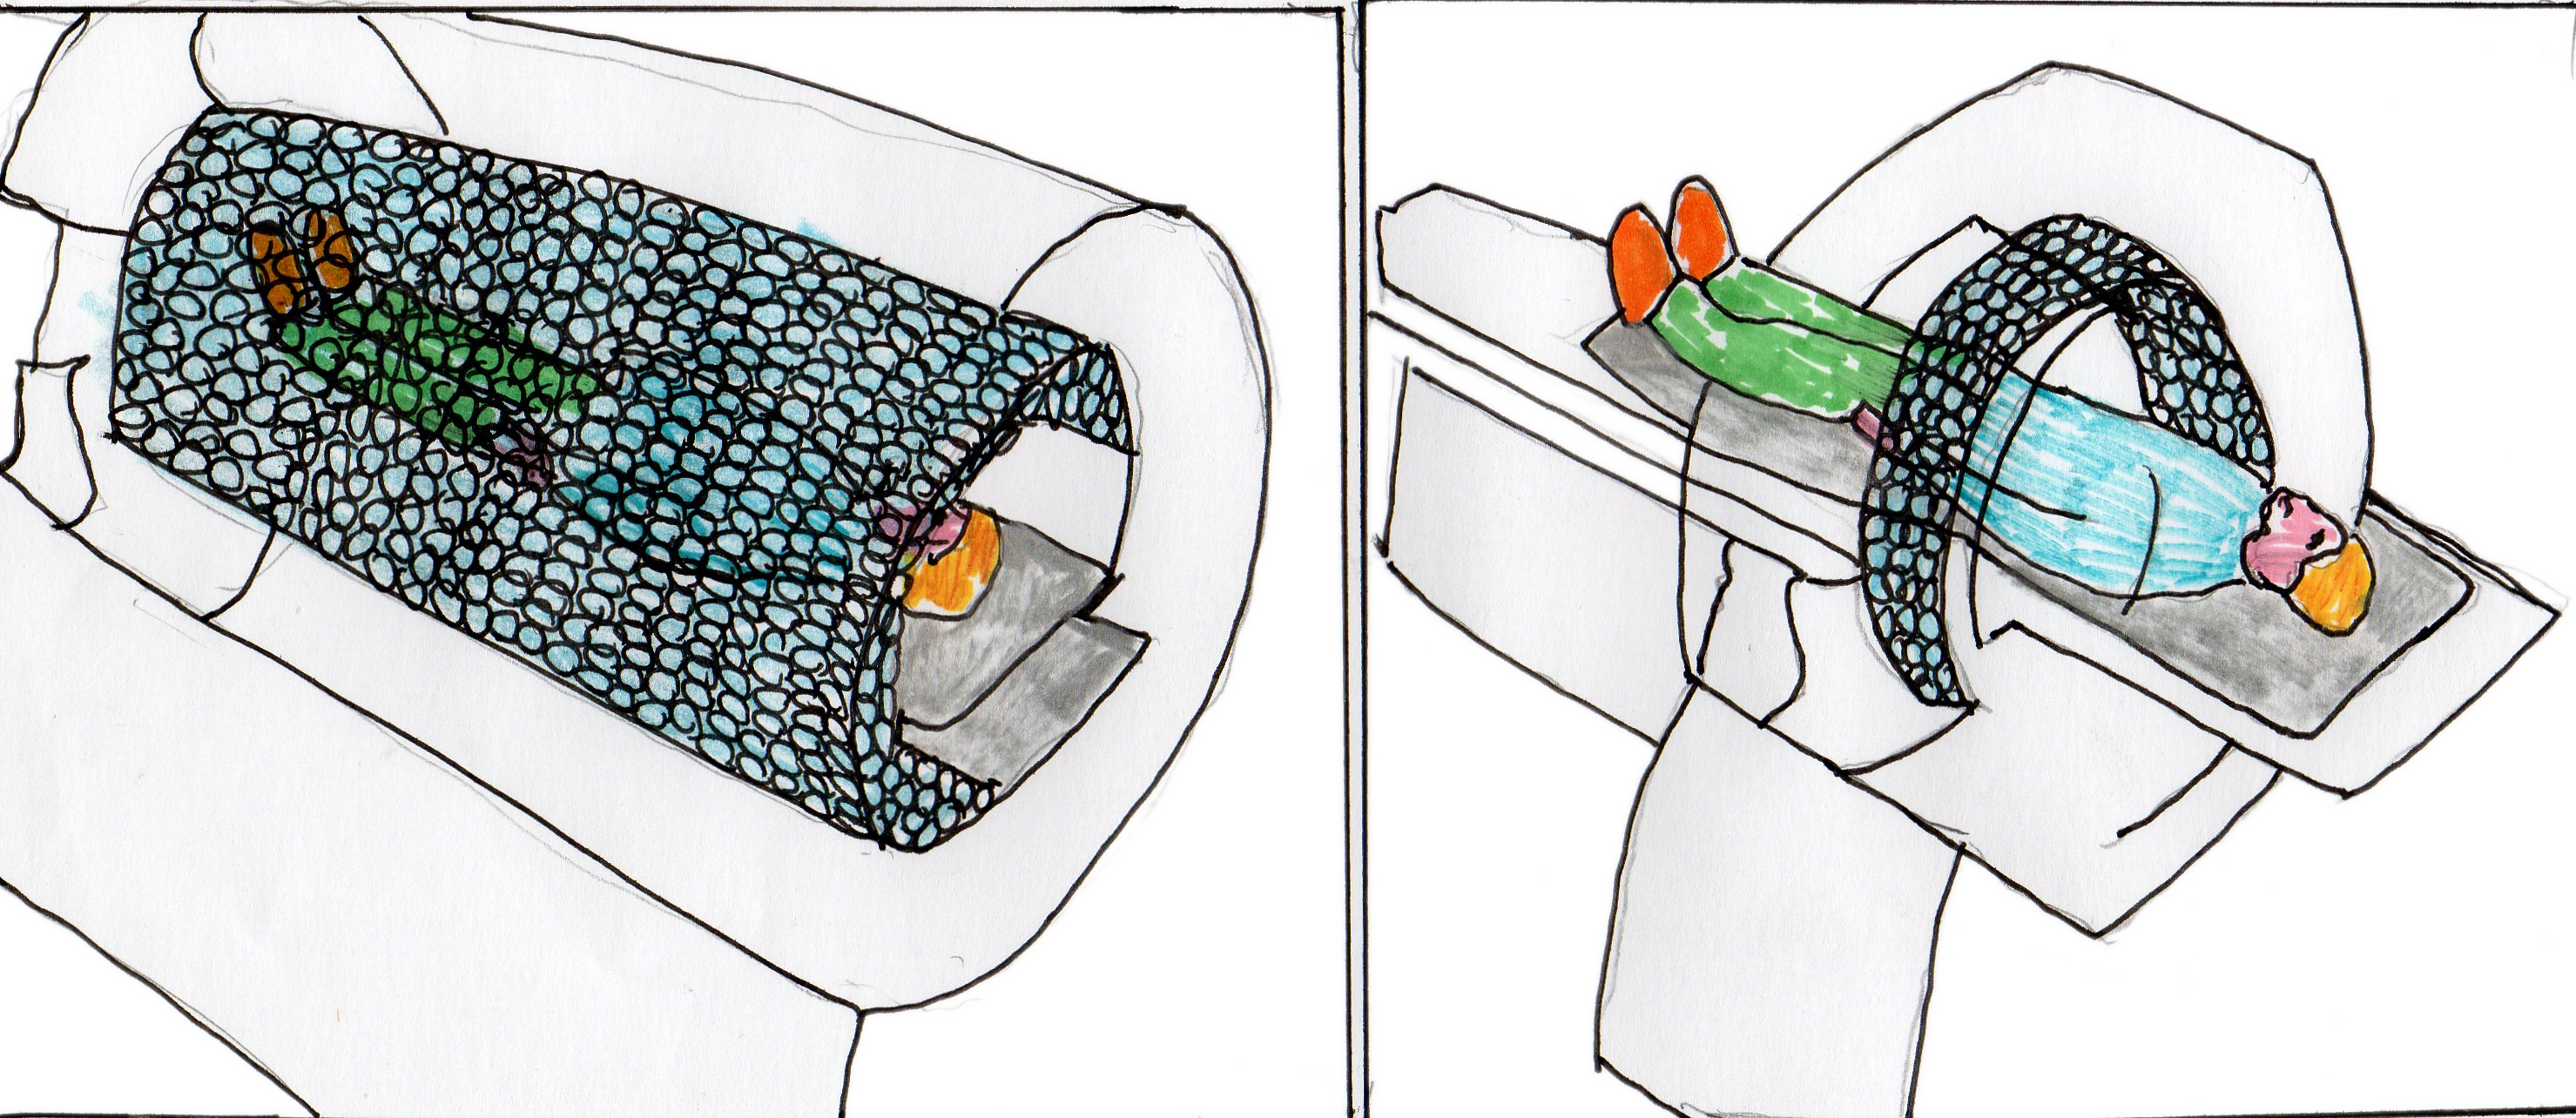
\includegraphics[width=1.0\linewidth]{figures/background_total_body_pet.png}
                    
                    \captionsetup{singlelinecheck=false, justification=raggedright}
                    \caption{Graphical representation of the difference between a total body \gls{PET} scanner and a standard \gls{PET} scanner. On the left of the figure a total body \gls{PET} scanner can be seen where the rings of detectors completely engulf the patient. However, on the right of the figure a standard \gls{PET} scanner can be seen where the rings of detectors only cover a portion of the patient. On the case on the right of the figure in order to take a scan over the entire body either individual acquisitions will be needed and concatenated or the bed would have to move while the acquisition was ongoing.} \label{fig:pet_fov_total_body_pet}
                \end{figure}
                
                The \gls{FOV} of the scanner is the area in which it can detect these $\gamma$-photons. Current clinical \gls{PET} scanners, usually, have a cylindrical \gls{FOV} with a length of between \SI{15.0}{\centi\metre} and \SI{25.0}{\centi\metre} and a diameter of between \SI{50.0}{\centi\metre} and \SI{70.0}{\centi\metre}~\boxcite{Pan2019}.
                
                There are multiple ways to acquire data over more than the axial length of scanner, three of these methods are:
                
                \begin{itemize}
                    \item The most simple and widely used method is to take acquisitions over multiple bed positions and concatenate them.
                    
                    \item A method which is still viable on standard axial length scanners is; to continually move the bed through the rings of the scanner while acquiring data. This allows, for instance, for the input function for dynamic scans to be acquired from the aorta before then moving to brain imaging or for scatter to be corrected for that come from outside the \gls{FOV}. A disadvantage of this though is that it introduces another source of motion to the acquisition from moving the bed, this makes standard motion correction much more difficult.
                    
                    \item Alternatively, total body \gls{PET} scanners are becoming more viable for research and have a high potential for clinical applications. Total body \gls{PET} scanners have an axial \gls{FOV} which contains most of the patients body making multiple acquisitions less necessary while also increasing the sensitivity to detecting annihilations, this can be seen in~\Fref{fig:pet_fov_total_body_pet}~\boxcite{Cherry2018}. However, the increased price and size constitute a limitation.
                \end{itemize}
            
            \subsubsection{Attenuation} \label{sec:attenuation}
                \begin{figure}
                    \centering
                    
                    \includegraphics[width=1.0\linewidth]{figures/background_scatter.png}
                    
                    \captionsetup{singlelinecheck=false, justification=raggedright}
                    \caption{Graphical representation of a $\gamma$-photon scattering off of a particle. The $\gamma$-photon can be seen entering the figure on the left hand side before scattering off of a particle in the centre of the figure by an angle $\theta$ and exiting the figure on the top right hand corner. The particle exits the scatter event with some velocity represented by the arrow towards the bottom right. The trajectory of the $\gamma$-photon, had it not been scattered, is shown by the dotted line on the right hand side of the figure.} \label{fig:attenuation_scatter}
                \end{figure}
                
                Attenuation is the amount of counts lost from annihilation to detection by the scanner while the photons are traversing through the body of the patient. Attenuation can amount to a loss of up to \SI{95.0}{\percent} of the total initial signal and can cause increased issues in larger bariatric patients who quite literally have more matter that the photons have to pass through increasing the likelihood that they will be scattered or otherwise attenuated~\boxcite{book, Essential2012}.
                
                There are four main ways through which the photon signal can be lost~\boxcite{book2}, these are in ascending order of magnitude:
                
                \begin{itemize}
                    \item Pair production can be thought of as the inverse process compared to annihilation (as discussed above). This is where a subatomic particle and its antiparticle, such as a electron and a positron, are created from a fundamental particle, such as a photon, usually in close proximity to an atomic nucleus. However, because of conservation of energy a photon would need to be of at least $1.022$ \gls{MeV} which is not generally possible for photons created through electron positron annihilation.
                    
                    \item Rayleigh scattering is the elastic scattering of photons without loss of significant energy by particles which are much smaller than the wavelength of the photon. A common example of Rayleigh scattering is the scattering of sunlight in the atmosphere which is causes the blue colour of the sky during the day and the red colour of the sky at sunset. Because the wavelength of $\gamma$-photons is comparably small, compared to most particles, the probability of Rayleigh scattering occurring is negligible and thus it is normally ignored in \gls{PET}.
                    
                    \item Absorption through the photoelectric effect is the process through which the high energy $\gamma$-photon hits and transfers its energy to a material causing the emission of lower energy electrons. The likelihood of the photoelectric effect is inversely proportional to the cube of the photon energy; it also increases as the atomic number of the attenuating material increases. In the matter of the patient the photoelectric effect is most prevalent at photon energies below $100$ \gls{KeV} and as such the probability of the photoelectric effect occurring here is minimal~\boxcite{book}. Photoelectric effect occurs mostly in the detectors of the scanner.
                    
                    \item Compton scattering comprises the majority of interactions between the photon and matter, it occurs where the photon interacts with an electron in a close by atom. The recoiling electron causes the photon to be deflected along another path transferring energy from photon to electron, this can be seen in~\Fref{fig:attenuation_scatter}. Compton scattering is also known as incoherent scattering because of its effect on the trajectory of the photon. The probability of Compton scattering is indirectly proportional to the energy of the photon~\boxcite{book}.
                \end{itemize}
                
                The relationship between the attenuation of the signal and the material through which it is travelling is given by the Beer-Lambert law. Given $I_0$ incident photons travelling across a path of length $D$, the number of non-attenuated photons $\rmI_{\rmD}$ is given by:
                 
                \begin{equation} \label{sec:eq:beer_lambert_law}
                    \rmI_{\rmD} := \rmI_{0} \cdot \exp\Bigg(\int_{\rmD} - \mu_E(r)\rmd r \Bigg)
                \end{equation}

                \noindent where $\mu_E(r)$ is the attenuation coefficient of the media crossed by the photons of energy $E$.
        
        \subsection{Data acquisition} \label{sec:data_acquisition}
            % write a general intro on the scanner structure, and the type of events you detect (true scatter randoms etc)
            
            \begin{figure}
                \centering
                
                \includegraphics[width=1.0\linewidth]{figures/background_coincidence.png}
                
                \captionsetup{singlelinecheck=false, justification=raggedright}
                \caption{Graphical representation of the different types of coincidences possible in \gls{PET}. On the left of the figure a true coincidence can be seen, this is where the $\gamma$-photons from one annihilation are both detected without scattering. In the middle of the figure a scattered coincidence can be seen, this is where the $\gamma$-photons from one annihilation are both detected, however in this case on of them has scattered. On the right of the figure a random coincidence can be seen, this is where the $\gamma$-photons from two unrelated annihilation are both detected.} \label{fig:data_acquisition_coincidence}
            \end{figure}
            
            As discussed in~\Fref{sec:pet_fov}, the structure of a \gls{PET} scanner is that of concentric rings of detectors offset along a central axis. These rings detect each incident photon and attempt to temporally and spatially link opposing photons along a \gls{LOR} through the scanner. The methods though which the scanner attempts to detect incident photons and then link relative photons together will be discussed in the following~\Fref{sec:photon_detection} and~\Fref{sec:coincidence_processing}.
            
            Because of the photons interaction in matter shown in~\Fref{sec:attenuation}, there are four different types of event or coincidences that can be detected by the scanner, these are:
            
            \begin{itemize}
                \item Firstly, the coincidences that originate from the same annihilation event and pass through the body of the patient to the detector without being scattered or attenuated. These coincidences are called true coincidences as they approximately accurately reflect the position of the originating annihilation.
                
                \item Secondly, there are coincidences, which may have originated from the same annihilation event but, from which one or more of the incident photons has undergone Compton scattering before detection. These coincidences are called scattered coincidences.
                
                \item Thirdly, there are coincidences where the \gls{LOR} is determined from two photons from two distinct annihilation events, thus the \gls{LOR} does not reflect an actual annihilation in reality. This could occur because one or more of the photons, from the original pair of photons, may have been attenuated or scattered so that it does not arrive at the detector within a reasonable time of its photon pair. These are called random coincidences.
                
                \item Fourthly, there could be a situation where three or more photons are detected within close temporal proximity to one another. Because of the close time of detection, in this case it is not possible to determine which photons reflect an actual annihilation and which are random coincidences. These coincidences are called multiple coincidences.
            \end{itemize}
            
            An example of some of the types of coincidences from above can be seen in~\Fref{fig:data_acquisition_coincidence}.
            
            The total prompts detected during a \gls{PET} acquisition $P$ can be expressed as:
            
            \begin{equation}
                P := T + S + R
            \end{equation}
            
            \noindent where $T$ is the number of true coincidences, $S$ is the number of scattered coincidences and $R$ is the number of random coincidences. Thus the usual total sum of scattered and random coincidences when compared to true coincidences is a ratio of $2$ to $1$.
            
            \subsubsection{2D and 3D Acquisition} \label{sec:2d_and_3d_acquisition}
                \begin{figure}
                    \centering
                    
                    \includegraphics[width=1.0\linewidth]{figures/background_septa.png}
                    
                    \captionsetup{singlelinecheck=false, justification=raggedright}
                    \caption{Graphical representation of the cross section of the septa used for collimation in \gls{2D} \gls{PET} acquisitions. In this figure a point can be shown casting paths into the slits of the septa, as can be seen the paths from the point can only pass through the slits of the septa in positions where the angle of the line with respect the the walls of the septa is acute.} \label{fig:2d_and_3d_acquisition_septa}
                \end{figure}
                
                There are two different methods used in \gls{PET} to determine or constrain to be certain of the spatial position or angle of the \gls{LOR} along the axis of the scanner, these are:
                
                \begin{itemize}
                    \item The method which was used for a long time in other applications (such as \gls{SPECT}) and until recently in \gls{PET} was; to place a block of, usually, tungsten metal (for its photon absorbing properties) in front of all of the detectors, this block is called s septa, this can be seen in~\Fref{fig:2d_and_3d_acquisition_septa}. The septa has very small slits cut into it which would only allow photons to pass through which entered the slits at an acute angle. Thus the septa constrains the photons to being almost perpendicular to the detector (on axis) and as such each detector only receives signal from annihilations that occur within its ring. This process is called collimation and the subsequent acquisition is called a \gls{2D} acquisition, \gls{2D} not because it results in a single image but because it is comprised of distinct \gls{2D} projections.
                    
                    \item The more modern method is to simply remove the septa from the scanner and to record coincidences between all rings. This is significantly more computationally expensive than a \gls{2D} acquisition but it also increases the sensitivity of the scanner meaning that scanning times can be reduced. Because this method produces projections between all rings it is known as a \gls{3D} acquisition~\boxcite{Schmitz2013}.
                \end{itemize}
            
            \subsubsection{Photon Detection} \label{sec:photon_detection}
                \begin{figure}
                    \centering
                    
                    \includegraphics[width=1.0\linewidth]{figures/background_detector.png}
                    
                    \captionsetup{singlelinecheck=false, justification=raggedright}
                    \caption{Graphical representation of the block detector structure of the scintillator crystal and the photodetector (with multiple scintillator crystals per photodetector), on the left of the figure, and an example of how these block detectors would be combined to construct a ring of a \gls{PET} scanner, on the right of this figure.} \label{fig:photon_detection_detector}
                \end{figure}
                
                \begin{figure}
                    \centering
                    
                    \includegraphics[width=1.0\linewidth]{figures/background_photomultiplier.png}
                    
                    \captionsetup{singlelinecheck=false, justification=raggedright}
                    \caption{Graphical representation of a scintillator crystal coupled to a \gls{PMT}. On the left of this figure a photon can be seen impinging upon the scintillator crystal and then being attenuated by the photoelectric effect at some depth. The electrons produced by this can then be seen, in the centre of this figure, interacting with the photocathode before being focused onto the first dynode. On the right of this figure, a naive representation, the amplification of the electrons can be seen by subsequent dynodes.} \label{fig:photon_detection_photomultiplier}
                \end{figure}
                
                PET detectors consist of two main components; a scintillator crystal, which, partially because of the photoelectric effect, when exposed to ionising radiation produces visible light through luminescence, and a photodetector or photomultiplier which amplifies the intensity of an input light similarly to how a vacuum tube or a transistor would amplify an electrical signal. These can be seen in~\Fref{fig:photon_detection_detector}.
                
                For use in \gls{PET} the following properties are desirable for a scintillator crystal:
                
                \begin{itemize}
                    \item Firstly, the crystal should have a high stopping power. This means that the photon does not travel a great distance into the crystal before it undergoes attenuation by the photoelectric effect. Usually the higher the density of the scintillator crystal the greater the stopping power.
                    
                    \item Secondly, for each incident photon the scintillator should have a high light output. This not only means that the work photomultiplier will have to amplify the output less but it also means that discriminating between scattered and unscattered photons will be easier as the discrepancy between the output intensity of the two will be greater.
                    
                    \item Thirdly, the scintillator should return to a state where it can luminesce again rapidly after each incident photon. This means that more photons can be detected over time and that the exact moment a photon is attenuated can be better measured.
                    
                    \item Finally, a scintillator crystal should not be hygroscopic. To be hygroscopic means that something has a tendency to absorb water.
                \end{itemize}
                
                The first \gls{PET} scanners used \gls{NaI} scintillator crystals before moving to \gls{BGO} and then to \gls{LSO} and \gls{LYSO}. Each new generation of scintillator crystals provided a different balance of the above characteristics. \gls{LSO} and \gls{LYSO} have the best combination of efficiency and time resolution while not being hygroscopic~\boxcite{BGOCherenkovBib, ScintilatorsBib, Mao2013CrystalCrystals}.
                
                There are three main types of photodetector or photomultiplier, these are:
                
                \begin{itemize}
                    \item The first kind of photodetector to be used in \gls{PET} was the \gls{PMT}, this device functions using an initial photocathode and a focusing electrode which takes the output from the scintillator and directs it towards a chain of dynodes. Dynodes are an intermediate electrode which when struck by a photoelectron emit more photoelectrons at a more positive electrical potential through secondary emission. Each subsequent dynode is a a higher potential and emits more photoelectrons than the last causing the input signal to be amplified, this can be seen in~\Fref{fig:photon_detection_photomultiplier}. Some disadvantages of \gls{PMT} are that they are relatively bulky, are effected by a magnetic field and have a relatively low efficiency at approximately \SI{25.0}{\percent}~\boxcite{book, SiPmBib}.
                    
                    \item To attempt to combat the low efficiency mentioned above the \gls{APD} was developed, this device utilises a semiconductor where there is a junction between positive and negative type silicone, this is similar to a traditional diode. This allows for efficiencies approaching \SI{85.0}{\percent}, they are much smaller than \gls{PMT} and are safe to be used in a magnetic field. However, this also comes with the drawbacks that \gls{APD} produces so much heat that it requires an active cooling system and exhibits worse timing characteristics than the \gls{PMT}~\boxcite{AvalanchePhotodiodeBib}. \gls{APD} is the choice of many modern \gls{PET}/\gls{CT} scanners~\boxcite{Vandendriessche2019}.
                    
                    \item A further development on \gls{APD} gave \gls{SiPM} and \gls{SSPM}. These devices combine the benefits of both \gls{PMT} and \gls{APD} in that they have a high efficiency, small size, are safe to be used in a magnetic field and have good timing characteristic. \gls{SiPM} and \gls{SSPM} are becoming the new default photodetectors in \gls{GE} scanners~\boxcite{SiPmBib}.
                \end{itemize}
            
            \subsubsection{Coincidence Processing} \label{sec:coincidence_processing}
                % write stuff about coincidence processing , give some info on TOF (or separate section for it, i don't know)
                
                \begin{figure}
                    \centering
                    
                    \includegraphics[width=1.0\linewidth]{figures/background_coincidence_processing.png}
                    
                    \captionsetup{singlelinecheck=false, justification=raggedright}
                    \caption{Graphical representation of the workflow from annihilation, to physical detection by the scanner, to then coincidence processing by the electronics of the scanner, before finaly displaying some output to the user.} \label{fig:coincidence_processing_coincidence_processing}
                \end{figure}
                
                In order for a \gls{LOR} to be determined, the annihilation from which pairs of detected photons come from must be determined, ie they must be paired together in some way, as briefly mentioned above in~\Fref{sec:data_acquisition}. First, before pairing, the photons are filtered by selecting ones which only fall within an energy window of the scanner, for the \gls{GE} Discovery 690/710 \gls{PET}/\gls{CT} this energy window fall approximately between $425$ and $600$ \gls{KeV}~\boxcite{Bettinardi2011}. Additionally, to attempt to determine temporally if two detected photons belong to the same annihilation event a coincidence window is used. If the events arrive more than the time of the coincidence window apart then they are determined to be unrelated. A standard coincidence window size would be about \SI{5.0}{\nano\second}. A naive representation of the workflow for coincidence processing can be seen in~\Fref{fig:coincidence_processing_coincidence_processing}.
            
            \subsubsection{Time of Flight PET} \label{sec:time_of_flight_pet}
                \begin{figure}
                    \centering
                    
                    \includegraphics[width=1.0\linewidth]{figures/background_tof.png}
                    
                    \captionsetup{singlelinecheck=false, justification=raggedright}
                    \caption{Graphical representation of the concept of \gls{TOF}. The top middle of this figure shows the position where a hypothetical annihilation has occurred, plus the $\gamma$-photos from this annihilation which have then gone on to be detected by the scanner. The bottom left of this figure shows a traditional \gls{NTOF} acquisition where the probability of the position of the annihilation along the \gls{LOR} is constant. The bottom right of this figure shows a \gls{TOF} acquisition where the probability of the position of the annihilation along the \gls{LOR} can be approximated with a Gaussian based upon the difference in arrival time of both photons.} \label{fig:time_of_flight_pet_tof}
                \end{figure}
                
                \begin{figure}
                    \centering
                    
                    \includegraphics[width=1.0\linewidth]{figures/background_non_tof_example.png}
                    
                    \captionsetup{singlelinecheck=false, justification=raggedright}
                    \caption{Example of some \gls{NAC} \gls{NTOF} data, with noise, with no motion, randoms or scatters, of the thorax with a spherical lesion in the lungs. Coronal view.} \label{fig:time_of_flight_pet_non_tof_example}
                \end{figure}
                
                \begin{figure}
                    \centering
                    
                    \includegraphics[width=1.0\linewidth]{figures/background_tof_example.png}
                    
                    \captionsetup{singlelinecheck=false, justification=raggedright}
                    \caption{Example of some \gls{NAC} \gls{TOF} data, with noise, with no motion, randoms or scatters, of the thorax with a spherical lesion in the lungs. Coronal view.} \label{fig:time_of_flight_pet_tof_example}
                \end{figure}
                
                As stated above in~\Fref{sec:coincidence_processing}, in order for the coincidence window based method to determine which specific detected photons represent \gls{LOR}, the scanner must be able to asses the difference in arrival time of each photon. Because of this the scanner must record the absolute time at which it detects each incident photon. It had been hypothesised for some time (since the 1960s) that given the speed of light and the difference in arrival time at each detector, for each photon that makes a specific \gls{LOR}, then it should be possible to approximately calculate the position upon the \gls{LOR} at which a given annihilation occurred, known as \gls{TOF}. This can be seen in~\Fref{fig:time_of_flight_pet_tof}~\boxcite{Surti2015, TOFPhotodetectorsBib}.
                
                The reason for the uncertainty of the position along the \gls{LOR} is because of the relatively course timing resolution of each given scanner. Generally modern \gls{PET}/\gls{CT} scanners have a timing resolution ranging between \SI{200.0}{\pico\second} and \SI{600.0}{\pico\second}, which represents an approximate spatial uncertainty of between \SI{60.0}{\milli\metre} and \SI{180.0}{\milli\metre}. The uncertainty within these \gls{TOF} bins is usually modelled using a Gaussian distribution centred around the estimated position of annihilation by the scanner.
                
                The timing resolution of the scanner is mainly dictated by the timing properties of both the scintillation crystal and the photodetector used. For the scintillation crystal, almost ubiquitously \gls{LSO} and \gls{LYSO} are used in modern \gls{PET} scanners which utilise \gls{TOF}. This is because they are the only scintillation crystals where they stop the photon and return to their base state post luminescence in a suitable time such that the time of arrival can be determined to any useful degree~\boxcite{TOFLSOBib}. For the photodetector, though \gls{PMT} possessed suitable timing properties to be used for \gls{TOF} now \gls{SiPM} and \gls{SSPM} are suppassing \gls{PMT} both in their timing properties and because they are not affected by magnetic fields and such can be used in both \gls{PET}/\gls{CT} as well as \gls{PET}/\gls{MR} scanners.
                
                Currently, \gls{TOF} is a focus for research because of the drastic improvements that it can have on the \gls{SNR}~\boxcite{Lecoq2017, Cates2018}. \gls{TOF} has such an impact on the resolution and reconstruction of \gls{PET} that it is used as a pseudo attenuation correction technique outside of the \gls{FOV} of the \gls{MR} in some \gls{PET}/\gls{MR} systems, such as the \gls{GE} Signa~\boxcite{Pan2019}. An example of some \gls{NAC} \gls{NTOF} and \gls{NAC} \gls{TOF} data can be seen in~\Fref{fig:time_of_flight_pet_non_tof_example} and~\Fref{fig:time_of_flight_pet_tof_example} respectively, notice the difference in distribution of counts in the centre of the thorax and lungs.
                
                The \gls{PET}/\gls{CT} scanner with the highest \gls{TOF} resolution which is commercially available is the Siemans Vision with an approximate \gls{FWHM} of \SI{210.0}{\pico\second} or \SI{63.0}{\milli\metre}~\boxcite{VanSluis2019}. The \gls{PET}/\gls{MR} scanner with the highest \gls{TOF} resolution which is commercially available is the \gls{GE} Signa with an approximate \gls{FWHM} that is sub \SI{400.0}{\pico\second} or \SI{120.0}{\milli\metre}~\boxcite{SIGNA, Hsu2017StudiesSystem, Grant2016NEMASystem, Caribe2019NEMAIsotopes}.
            
            \subsubsection{Data Output} \label{sec:data_output}
                \begin{figure}
                    \centering
                    
                    \includegraphics[width=1.0\linewidth]{figures/background_projection_data_example.png}
                    
                    \captionsetup{singlelinecheck=false, justification=raggedright}
                    \caption{Example of some simulated projection data, with no motion, noise, randoms or scatters, of the thorax with a spherical lesion in the lungs.} \label{fig:data_output_projection_data_example}
                \end{figure}
                
                The output from a \gls{PET} scanner must be stored in a universally understood file format in order to be of any use. This file format will usually contain information related to the prompts from the acquisition, discussed above in~\Fref{sec:data_acquisition}. Each prompt stored represents a \gls{LOR} connecting the centre of two detectors, where \gls{TOF} information is available it is stored as an extra dimension in this file. This file can then be taken and reconstructed in order to estimate the original distribution of the radiotracer in the patient, this will be discussed later in~\Fref{sec:pet_image_reconstruction}. The data output from a \gls{PET} scan are usually expressed in \gls{kBq/mL}, however for pseudo quantitative analysis the values are usually normalised to \gls{SUV} by dividing the activity by, for instance, the mass of the patient and the injected activity.
                
                There are two main formats in which this information is stored from the scanner, these are:
                
                \begin{itemize}
                    \item The most common way, that is used in clinical practise, is a format called a sinogram. During acquisition, if a sinogram output is specified, then the coincidences detected by the scanner are binned into a histogram which represents their plane orthogonal to the scanner, their orientation angle, their average axial location and their distance from the centre of the gantry. If a single point source were imaged it would produce a sinusoid when binned into a sinogram, hence the name. An example of some projection data, with no noise, can be seen in~\Fref{fig:data_output_projection_data_example}. Because data is being binned into a histogram with this method then information is lost, it could be considered a lossy compression method.
                    
                    \item A less common method but one which is becoming more prevalent is a format called listmode data. Here each coincidence is recorded sequentially in a file. The information stored for each coincidence includes its arrival time, the coordinates of the detector and coincidence and its detected energy. A listmode file can be directly reconstructed or unlisted into a sinogram post acquisition. Because a listmode file does not compress the output from the scanner, such as by binning the data into a histogram like with a sinogram, then the size of a listmode file will always be inherently larger than an equivalent sinogram.
                \end{itemize}
            
            \subsubsection{PET resolution} \label{sec:pet_resolution}
                There are five main effects which impact the resolution of a \gls{PET} acquisition, these are:
                
                \begin{itemize}
                    \item Firstly, there is, as has been discussed above in~\Fref{sec:decay_and_annihilation}, the effect of positron range. Because the positron travels a small distance before annihilating the \gls{PET} scanner will always, at best, be measuring the position of the annihilation rather than the position of the decay and as such not directly measuring the position of the radiotracer~\boxcite{PositronRangeLevinHoffmanBib}.
                    
                    \item Secondly, again as discussed above in~\Fref{sec:attenuation}, because the positron will almost always enter the annihilation event with some velocity then the $\gamma$-photons produced will exit with the same additional velocity. This velocity is also almost always in a direction other than that which the $\gamma$-photon would otherwise travel in, this causes the photons to travel in a direction which is not exactly $\SI{180}{^{\circ}}$ apart from one another. This effect is exacerbated by the amount of time that the photons are allowed to travel, thus the larger the bore of the \gls{PET} scanner the larger this effect will have on the resolution. The effect of acolliniarity on \gls{F-FDG} gives an error of approximately $\SI{0.54}{^{\circ}}$~\boxcite{AccollinearityBib}
                    
                    \item Thirdly, the size of each detector dictates the angular resolution of the scanner, or the number of \gls{LOR} covering any $\SI{360}{^{\circ}}$ slice is directly proportional to the number of detectors in each ring. Thus the resolution at which you can reconstruct before the sparsity of the \gls{LOR} means that some voxels will have zero \gls{LOR} passing through them is determined by the size of each individual detector~\boxcite{Nieman2015}.
                    
                    \item Fourthly, The block construction of each detector negatively impacts the resolution. This is because a number of scintillation crystals is paired with, usually, fewer photodetectors, this can be seen in~\Fref{fig:photon_detection_detector}. This means if a photon interacts with one crystal it may incorrectly be attributed to another crystal~\boxcite{Nieman2015}. So called digital \gls{PET} scanners are beginning to be seen which use a $1:1$ ratio of photodetectors to scintillation crystal, effectively removing issues related to block construction~\boxcite{Schillaci2019DigitalImaging}.
                    
                    \item Finally, as discussed in~\Fref{sec:photon_detection}, a scintillation crystal has some stopping power, this power describes the approximate depth at which photons will undergo attenuation by the photoelectric effect. In some instances, depending upon the position and angle at which the incident photon hits the scintillation crystal it is possible for the photon to travel through the crystal and into an adjacent crystal before being detected. This means that the photon is incorrectly positioned and will result in blurring of the reconstructed volume~\boxcite{Nieman2015}.
                \end{itemize}
        
        \subsection{Combined PET/CT} \label{sec:combined_pet_ct}
            A \gls{CT} scanner consists of two straight parallel devices which sit one on either side of the bore of the scanner. One device is an X-ray emitter and the other is an X-ray detector. If the X-ray emitter were to operate in one fixed position the result would be similar to a standard diagnostic X-ray, the difference comes in that for \gls{CT} during a continuous acquisition the device spins around the axis of the scanner taking continuous measurements. This allows for an X-ray image at every angular position. While spinning the \gls{CT} scanner also travels along the axis of the scanner, this allows for the collection of data over a \gls{3D} volume (as what \gls{PET} collects over).
            
            When the X-ray beam intersects with the body of a patient it is possible for the beam to be attenuated by the photoelectric effect, similarly to discussed in~\Fref{sec:attenuation}. Where the intensity of the beam detected is less it can be assumed that there is a more dense object attenuating more of the beam between it and the emitter. If this information is collected over a \gls{3D} volume it allows for the generation of a \gls{3D} volume that reflects the attenuation of the body of the patient, for instance. This attenuation is normally expressed in \gls{HU}.
            
            The energy of the X-ray used in \gls{CT} consists of many different wavelengths, or polychromatic. The wavelength range usually used in a \gls{PET}/\gls{CT} acquisition is between $40$ and $140$ \gls{KeV}~\boxcite{CTattenuationenergyBib}. The wavelength range is determined by the settings of the scanner, these mainly consist of the peak \gls{kVp} and the electric current applied, in milliamps.
            
            In a standard \gls{PET}/\gls{CT} scan the \gls{CT} component comes first before the \gls{PET}. In modern \gls{PET}/\gls{CT} scanners the \gls{CT} and \gls{PET} are inline one the same bed, however the first \gls{PET}/\gls{CT} scans were taken on different machines entirely and as such the position of the patient differed more drastically between scans. A standard \gls{CT} scan over the thoracic region will last approximately between \SI{2.0}{\second} and \SI{3.0}{\second}~\boxcite{PETCTImagingTechnicalConsiderationsBib}.
        
            \subsubsection{Attenuation Correction} \label{sec:attenuation_correction}
                \begin{figure}
                    \centering
                    
                    \includegraphics[width=1.0\linewidth]{figures/background_mu_map_example.png}
                    
                    \captionsetup{singlelinecheck=false, justification=raggedright}
                    \caption{Example of a simulated \gls{mu-map}, with no motion or noise, of the thorax with a spherical lesion in the lungs. Coronal view.} \label{fig:combined_pet_ct_mu_map_example}
                \end{figure}
                
                \begin{figure}
                    \centering
                    
                    \includegraphics[width=1.0\linewidth]{figures/background_nac_example.png}
                    
                    \captionsetup{singlelinecheck=false, justification=raggedright}
                    \caption{Example of simulated \gls{NAC} \gls{TOF} data, with motion, with no noise randoms or scatters, of the thorax with a spherical lesion in the lungs. Transverse view.} \label{fig:combined_pet_ct_nac_tof_example}
                \end{figure}
                
                \begin{figure}
                    \centering
                    
                    \includegraphics[width=1.0\linewidth]{figures/background_ac_example.png}
                    
                    \captionsetup{singlelinecheck=false, justification=raggedright}
                    \caption{Example of simulated \gls{AC} \gls{NTOF} data, with motion, with no noise, randoms or scatters, of the thorax with a spherical lesion in the lungs. Transverse view.} \label{fig:combined_pet_ct_ac_tof_example}
                \end{figure}
                
                As discussed previously in~\Fref{sec:attenuation} attenuation represents the loss of coincidences by photon interactions in matter. Attenuation is an issue in \gls{PET} as it causes the loss of signal and a degradation in image quality, this is the opposite for \gls{CT} where the modality itself relies on attenuation in order to differentiate anatomical structure, an example of a \gls{mu-map} can be seen in~\Fref{fig:combined_pet_ct_mu_map_example}. An example of some \gls{NAC} \gls{TOF} and \gls{AC} \gls{TOF} data can be seen in~\Fref{fig:combined_pet_ct_nac_tof_example} and~\Fref{fig:combined_pet_ct_ac_tof_example} respectively. In order to find reasonable quantitative results the attenuation of the patient must be taken into account in \gls{PET}. Both \gls{PET} and \gls{CT} follow the Beer-Lambert law.
                
                Methods to acquire \gls{mu-map}, for attenuation correction include; to take a transmission scan of a known point source rotated around the body of the  prior to the injection of the radiotracer. This allows for the estimation of the attenuation for each angle~\boxcite{TransmissionatnBib}. Another method involves the use of the known attenuation from the \gls{CT} scan.
                
                In order to apply the \gls{CT} based \gls{mu-map} to attenuation correction in \gls{PET} first it must undergo either bilinear or trilinear conversion to asses the attenuation coefficient factors, this is because of the relative energy difference of the two modalities~\boxcite{Carney2006}. As discussed above in~\Fref{sec:coincidence_processing} and~\Fref{sec:combined_pet_ct} \gls{PET} and \gls{CT} operate at two different energy levels of between between $425$ and $600$ \gls{KeV} and between $40$ and $140$ \gls{KeV} respectively~\boxcite{Bettinardi2011, CTattenuationenergyBib}.
                
                Issues with \gls{CT} based attenuation correction include: Firstly, as mentioned above in~\Fref{sec:combined_pet_ct}, \gls{CT} is acquired sequentially to \gls{PET} rather than simultaneously meaning that there can be mismatches in anatomy between the scans. Secondly, the propagation of any artefacts from the \gls{CT} volume into the \gls{PET} volume. Regardless of these issues \gls{CT} is currently considered to be the gold standard for \gls{mu-map} estimation for attenuation correction. Transmission scans are now very rarely used because of their sensitivity to user error, inclusion of an additional external source and their significant increase in scan time.
    
    \longsection{Inverse Problems and Optimisation}{sec:inverse_problems_and_optimisation}
        
        
        \subsection{Inverse Problem Concepts} \label{sec:inverse_problem_concepts}
            An inverse problem is one where the original conditions of a system are attempted to be derived from the effects of the system. For instance, the data from a \gls{PET} scanner represents the observations of the distribution of the radiotracer in the patient, reconstruction is an attempt to find the distribution from these observations.
            
            Because it is not usually possible to directly invert to find the solution, because of the size of a given matrix for instance causing the computation time to find an inverse to be large, then the solution must be optimised for. In order to attempt to find the solution to an inverse problem there are two things which are required; first the forward operator is required which is the inverse of the inverse problem, which is being solved, or the forward problem, second, at least, a model of the noise present in the system is required.
        
        \subsection{Optimisation Concepts} \label{sec:optimisation_concepts}
            Optimisation means to find some values that best paramatarise some given function. For instance, in reconstruction an optimisation could be to find the image that when it has the forward operator applied to it best matches the measured data. Another example of an optimisation would be to find the motion parameters that when applied to a given image most closely warp that image to match another image. Optimisation is also used in fields such as when training neural networks, here the optimisation finds parameters for a model that maps one set of values to another, this will be discussed later in~\Fref{sec:machine_learning_for_pet}.
            
            In order to perform a basic optimisation there are two things which are required; first an objective function to optimise is requires and then a method to optimise some given values based on this function is required, these will be discussed in the following sections in~\Fref{sec:objective_function} and~\Fref{sec:optimiser} respectively.
        
        \subsection{Objective Function} \label{sec:objective_function}
            Optimisation of some values requires a function that represents, for instance, the similarity of two measures or the likelihood of something given a measure. This function is required because in a sense the optimiser attempts to find some solution by either maximising or minimising the result of applying this function iteratively until either a maximum number of iterations or some other stopping criteria is reached.
            
            An example of an objective function would be \gls{MAE}. For a vector of some values, \gls{MAE} subtracts the estimated value from the true value, finds the absolute of this, sums together this value for all values in the vector and divides by the number of values in the vector. The absolute value is taken because the error should be the distance to the true value regardless of if the estimated value is greater or less than the true value. This method finds the mean error over all estimated values. If the estimated values approach the true values then the value of the \gls{MAE} will approach zero in a linear fashion. If \gls{MSE} is used then rather than taking the absolute of the error the square is taken instead, taking the square causes the error to increase exponentially as it becomes larger. \gls{MAE} and \gls{MSE} are usually used in regression like problems where a line is fit though a data set.
            
            Another example of an objective function would be likelihood. This function for any given sample of data returns the goodness of fit to a statistical model. The likelihood function describes a planes whose peak, if there is one distinct peak, represents the values which maximises the probability of drawing the sample obtained~\boxcite{Myung2003TutorialEstimation}. \gls{MLE} is often used in \gls{PET} image reconstruction.
            
        \subsection{Optimiser} \label{sec:optimiser}
            \begin{figure}
                \centering
                    
                \includegraphics[width=1.0\linewidth]{figures/background_optimisation.png}
                    
                \captionsetup{singlelinecheck=false, justification=raggedright}
                \caption{Graphical representation of a \gls{2D} solution space and an optimiser stepping through this space. In the bottom left of this figure the initial estimate for some optimisation can be seen at $x$, the subsequent iterations $1$ through $4$ can then be seen taking this estimate closer to the centre of the contour plot. Here the contour plot could either be showing a maximisation or a minimisation depending on how it is visualised.} \label{fig:optimiser_optimisation}
            \end{figure}
            
            The optimiser takes an initial estimate of the values that are to be optimised and at least a function to either minimise or maximise the output of with the input of the estimate. This can be seen in~\Fref{fig:optimiser_optimisation}. The method by which the optimiser goes about updating the value of the estimate is what differentiates most optimisation algorithms.
            
            \gls{GD} is a commonly used optimisation algorithm. \gls{GD} attempts to find the gradient of the objective function over time and takes steps, of a given size, through the plane of the estimate in the direction calculated from the gradient which most shrinks the value of the objective function. The step size of \gls{GD} can be set to a fixed value or found using a line search which optimises the step size. Momentum can be used in \gls{GD} where the current update direction is linear combination, with a predefined weighting, of the current gradient and the previous update direction. Momentum attempts to reduce the effect of local minimum solutions or non-convex solution spaces by reducing the likelihood of the current update causing the optimisation to jump back and forth between two close values. 
            
            \gls{SGD} is an extension of \gls{GD} where the current update is calculated using the gradients of a randomly selected subset of the estimate, this is significantly more computationally efficient that \gls{GD} as it reduces the number of calculations needed for each update.
            
            \gls{CG} is another extension of \gls{GD}, here the direction of subsequent updates are confined so that they are orthogonal to the previous update direction, this can decrease convergence time as it can avoid the same issues as momentum~\boxcite{Tustison2009}.
            
    \longsection{PET Image Reconstruction}{sec:pet_image_reconstruction}
        
        
        \subsection{Analytic Image Reconstruction} \label{sec:analytic_image_reconstruction}
            % mention briefely FBP ?
            \begin{figure}
                \centering
                    
                \includegraphics[width=1.0\linewidth]{figures/background_radon_transform.png}
                    
                \captionsetup{singlelinecheck=false, justification=raggedright}
                \caption{Graphical representation of the Radon transform for one angle $\theta$. The Radon transform computes projections of some data along specified directions. Here, this figure shows the computation of a set of line integrals for the function $f(x, y)$, usually from multiple sources of parallel beams. To form a full image the Radon transform rotates the source around the centre of the image. This figure specifically shows projections for a simple \gls{2D} image along horizontal and vertical components $x$ and $y$.} \label{fig:analytic_image_reconstruction_radon_transform}
            \end{figure}
            
            \begin{figure}
                \centering
                
                \includegraphics[width=1.0\linewidth]{figures/background_bp_example.png}
                
                \captionsetup{singlelinecheck=false, justification=raggedright}
                \caption{Example of a simulated \gls{AC} \gls{NTOF} \gls{BP} reconstruction, with motion and noise, with no randoms or scatters, of the thorax with a spherical lesion in the lungs. Transverse view.}
                \label{fig:analytic_image_reconstruction_bp_example}
            \end{figure}
            
            \begin{figure}
                \centering
                
                \includegraphics[width=1.0\linewidth]{figures/background_fbp_example.png}
                
                \captionsetup{singlelinecheck=false, justification=raggedright}
                \caption{Example of a simulated \gls{AC} \gls{NTOF} \gls{FBP} reconstruction, with motion and noise, with no randoms or scatters, of the thorax with a spherical lesion in the lungs. Transverse view.}
                \label{fig:analytic_image_reconstruction_fbp_example}
            \end{figure}
            
            An analytic solution is one which offers a direct mathematical method through which one thing can be transformed to another. All analytical solutions can have a proof. An analytical solution for \gls{PET} reconstruction is \gls{BP}, in \gls{2D} \gls{BP} is the inverse Radon transform. This can be seen in~\Fref{fig:analytic_image_reconstruction_radon_transform}. To apply the inverse Radon transform to a \gls{2D} sinogram; first the rows of the sinogram, corresponding to $\SI{0}{^{\circ}}$ through $\SI{180}{^{\circ}}$, are taken individually and have the Fourier transform applied to them. Then the result of this is reshaped to polar coordinates so that each row is the diameter of a circle and a \gls{2D} Fourier transform is applied giving the final output image. The Fourier transform decomposes a function into its constituent frequencies. The \gls{2D} Fourier transform of a function computed along a line is equivalent to the 1D Fourier transform of the Radon transform along that line. This is called projection slice theorem. 
            
            \gls{FBP} was proposed as a solution to some of the issues apparent in \gls{BP}, like the fact that \gls{BP} suffers from low frequency blurring. In \gls{FBP} a high pass ramp filter is applied to the sinogram before it is Fourier transformed, thus removing some low frequency information or blurring. A low pass ramp filter can also be applied at the same time which removes some high frequency information or noise, this then would be a band pass filter. An example of a \gls{BP} and \gls{FBP} reconstruction can be seen in~\Fref{fig:analytic_image_reconstruction_bp_example} and~\Fref{fig:analytic_image_reconstruction_fbp_example}. Because of its speed and good quantitative results \gls{FBP} was the gold standard of \gls{PET} image reconstruction, however because of the issues mentions above it has now almost entirely been replaced by iterative reconstruction methods. \gls{FBP} is now almost solely used in longitudinal studies which started before the use of iterative reconstruction methods became prevalent~\boxcite{FBPReviewBib, PETCTReviewBib}.
            
            \gls{BP} and \gls{FBP} reconstruct a low quality image but are computationally fast. \gls{BP} will usually result in there being numerous streak like artefacts in the output image, the artefacts are exacerbated as noise increases. Artefacts can be caused because neither \gls{BP} nor \gls{FBP} account for the stochastic nature of the acquisition process, neither do they account for other factors such as positron range as discussed in~\Fref{sec:attenuation}.
            
            
        \subsection{Iterative Image Reconstruction} \label{sec:iterative_image_reconstruction}
            \begin{figure}
                \centering
                
                \includegraphics[width=1.0\linewidth]{figures/background_osem_example.png}
                
                \captionsetup{singlelinecheck=false, justification=raggedright}
                \caption{Example of a simulated \gls{AC} \gls{NTOF} \gls{OSEM} reconstruction, with motion and noise, with no randoms or scatters, of the thorax with a spherical lesion in the lungs. Transverse view.}
                \label{fig:iterative_image_reconstruction_osem_example}
            \end{figure}
            
            As discussed above in~\Fref{sec:inverse_problems_and_optimisation} an inverse problem, which \gls{PET} reconstruction is, can be solved by an iterative optimisation problem. In order to implement an iterative optimisation problem a few criteria must first be met; a forward operator which takes an image and return the projections which would result from acquiring the image is required. As discussed above in~\Fref{sec:optimisation_concepts} an objective function to assess the accuracy of the fit and an optimisation algorithm to improve the fit are required. Also, an initial estimate, which could be a volume the size of the output image filled with ones or zeros, and some method to cease execution, for instance stopping when the objective function reaches a certain value or the number of iterations exceeds a threshold, are also necessary.
            
            An iterative method has the advantage that the model which is used can take into account the noise properties of the data and also the physical properties of the scanner itself. The noise associated with \gls{PET} is often assumed to be Poisson distributed. However, iterative methods have the disadvantage that because they are often significantly complex then they require substantial computational effort to execute which will increase computation time when compared to analytical reconstruction.
            
            \gls{ML} is a commonly used objective function for iterative \gls{PET} reconstruction, this builds on the concepts, specifically \gls{MLE}, mentioned in~\Fref{sec:objective_function}. When maximising the likelihood the natural logarithm of the likelihood, also known as the log-likelihood, is often taken for computational efficiency. \gls{ML} is often combined with the \gls{EM} algorithm for the optimisation of the model parameters and in this case is called \gls{MLEM}~\boxcite{MLEMBib,PETMLEMBib,PETMLEM2Bib}. The output from \gls{MLEM} commonly has a Gaussian blur applied in order to attempt to smooth noise~\boxcite{PETMLEMFiltBib}. Disadvantages associates with \gls{MLEM} include, that for noisy data iterating for too long can cause the output to accentuate the noise present in the data, one way to avoid this is to purposefully cease iterating early before the noise can take over the image~\boxcite{PETMLEMTerminationBib}. Another issue, as mentioned earlier, is that \gls{MLEM} is exceptionally slow even when compared to other iterative algorithms, as will be discussed below.
            
            To combat the slow execution speed of \gls{MLEM} \gls{OSEM} was developed. In \gls{OSEM} \gls{LOR} or detector pairs of the scanner are binned into a number of subsets, in \gls{MLEM} there would be one subset and \gls{MLEM} would be applied to all \gls{LOR} or detector pairs simultaneously. However, in \gls{OSEM} the \gls{LOR} or detector pairs would be binned into at lease two subsets and then \gls{MLEM} would be applied to each subset, in a specific order, sequentially~\boxcite{OrderedSubsetsHudsonBib, OrderedSubsetsHuttonBib}. Because the image is updated after each iteration of \gls{MLEM} on each subset of \gls{OSEM} then the execution speed of \gls{OSEM} is increased by the number of subsets used. However, if more than two subsets are used then then \gls{OSEM} will converge to a limit cycle around true convergence~\boxcite{Mettivier2011}. If a reasonable number of subsets are used then it has been found that \gls{OSEM} will accelerate \gls{MLEM} without affecting the accuracy of quantification too drastically~\boxcite{Morey2013}. An example of an \gls{OSEM} reconstructed image can be seen in~\Fref{fig:iterative_image_reconstruction_osem_example}.
            
    \longsection{Respiratory Motion in PET}{sec:respiratory_motion_in_pet}
        % general intro
        
        \subsection{Respiratory Motion Artefacts} \label{sec:respiratory_motion_artefacts}
            % have a look at https://www.sciencedirect.com/science/article/pii/S0001299808000214?via%3Dihub
            
            \begin{figure}
                \centering
                
                \includegraphics[width=1.0\linewidth]{figures/background_motion_artefact_example.png}
                
                \captionsetup{singlelinecheck=false, justification=raggedright}
                \caption{Example of a simulated \gls{AC} \gls{NTOF} \gls{OSEM} reconstruction, with motion, with no noise, randoms or scatters, of the thorax with a spherical lesion in the lungs. Coronal view.}
                \label{fig:respiratory_motion_artefacts_motion_artefact}
            \end{figure}
            
            \begin{figure}
                \centering
                
                \includegraphics[width=1.0\linewidth]{figures/background_single_mu-map_ac_example.png}
                
                \captionsetup{singlelinecheck=false, justification=raggedright}
                \caption{Example of a simulated single \gls{mu-map} \gls{AC} \gls{NTOF} \gls{OSEM} reconstruction, with motion, with no noise, randoms or scatters, of the thorax with a spherical lesion in the lungs. Coronal view.}
                \label{fig:respiratory_motion_artefacts_single_mu-map_ac}
            \end{figure}
            
            A single static bed position acquisition on a conventional \gls{PET} scanner takes approximately \SI{120}{\second}. This means that, because the patient is in respiratory motion throughout the acquisition, then the result of the scan will contain data from different respiratory phases. During the different respiratory phases the position and size of the lungs, diaphragm and any lesion will change. If the data is reconstructed all together then this will cause a blurring artefact especially prevalent around the anatomy that is moving the most, such as the diaphragm. This would be expected as the data, in this case, represents as if the respiratory phases had been summed together, an example of a \gls{PET} reconstruction with motion artefacts can be seen in~\Fref{fig:respiratory_motion_artefacts_motion_artefact}, notice the blurring above the diaphragm on the right side of the figure. Artefacts originating from the moving anatomy pose the largest challenge in imaging of the thorax~\boxcite{LungMotionArtefactBib, PETCTArtifactBib}.
            
            The artefacts caused by respiratory motion lead to issues clinically with cancer staging and follow up. This is because the size of the tumour is often over estimated and, because this causes the activity in the lesion to be spread out over more voxels, it also results in the activity being underestimated~\boxcite{LungMotionJudgmentErrorsBib}.
            
            If attenuation is corrected for then the position of this \gls{mu-map} in relation to the position of the \gls{PET} data also poses an issue. Where the \gls{mu-map} does not match the position of the anatomy then it will cause either under or over correction for attenuation, this causes a type of artefact often referred to as a banana artefact for the shape of the shadow that it causes to appear above the diaphragm~\boxcite{LungMotionDiaphragmBaiBib}. An example of this can be seen in~\Fref{fig:respiratory_motion_artefacts_single_mu-map_ac}, notice the black arc shaped artefact over the diaphragm and on the heart. The mismatch of the \gls{mu-map} and \gls{PET} data does not just cause this artefact but it can also change the expectation and thus the quantification of the reconstructed image will be affected. To combat intra-\gls{mu-map} motion the patient will often be asked to hold their breath, if they can, as the acquisition can only last between \SI{90}{\second} and \SI{150}{\second}~\boxcite{Nyflot}.
            
        \subsection{Respiratory Motion Challenges in Combined PET/CT Imaging} \label{sec:respiratory_motion_challenges_in_combined_pet_ct_imaging}
            To overcome the issues mentioned in~\Fref{sec:respiratory_motion_artefacts}, specifically related to the mismatch between \gls{mu-map} and \gls{PET} data a number of solutions have been proposed. Three such solutions which have been developed for \gls{CT} based \gls{mu-map} are:
            
            \begin{itemize}
                \item Firstly, a method which acquires \gls{PET} data over a prolonged acquisition and throws away any data where the patient is in a position other than the one that corresponds to the \gls{mu-map}. For this all data which is not at either one of full expiration or full inspiration would be removed~\boxcite{Liu2010, Grootjans2014}. Then the one breath hold \gls{CT} \gls{mu-map} would be warped to this data~\boxcite{LungMotionBreathHoldBib}. An advantage of this approach is that it not only would correct for the misalignment of \gls{mu-map} and \gls{PET} data but it would also eradicate any blurring associated with averaging over respiratory phases. A disadvantage is that, this solution would mean that either there would be substantially more noise in the reconstructed data (if the acquisition was the same length as a standard one) or the acquisition would need to take significantly longer, as so much data is being removed~\boxcite{Nehmeh2008a}. Additionally, dynamic scans would not be possible with this correction method. This is because the tracer kinetics could be shorter than one respiratory cycle and thus would be lost when those parts of the acquisition are removed.
                
                \item Secondly, a method similar to the first one has been proposed, this is where the \gls{PET} data is separated into individual images representing the separate respiratory phases. The one breath hold \gls{CT} \gls{mu-map} would then be warped in turn to each respiratory phase. This method provides the advantage over the first in that it uses all of the data from the \gls{PET} acquisition and provides a more robust reconstruction~\boxcite{4DPhaseMatchedReconBib}. A disadvantage is, that the reconstruction of each respiratory phase is likely to contain more noise than if all of the \gls{PET} data was reconstructed simultaneously. This is because the reconstruction algorithm is none linear and summing reconstructed volumes is not the same as summing projection data and then reconstructing. The higher levels of noise in the reconstructed data can pose a problem when attempting to warp the \gls{mu-map} to them.
                
                \item Finally, a method by where the reconstruction an motion parameters can be estimated simultaneously, directly from the \gls{PET}, for one breath hold \gls{CT} \gls{mu-map} has been recently proposed~\boxcite{JacobsonFesslerMotionCorrectionBib, Rezaei2012, Bousse2016a}. Here, the \gls{PET} data is split into the respiratory phases, as above. Then it is iterated between a reconstruction step and a motion parameter estimation step where the same parameters are used to warp both the \gls{PET} data and the \gls{mu-map} for each respiratory position. Thus the \gls{mu-map} does not have to correspond to any one respiratory phase as each set of \gls{PET} data will be reconstructed at the position of the \gls{mu-map}. This method works especially well when \gls{TOF} data is available~\boxcite{Bousse2016b}. A disadvantage of this method is that it takes more computation than the above methods and that because it has only recently started to be used then it has not been as extensively evaluated.
            \end{itemize}
    
    \longsection{Motion Correction for PET}{sec:motion_correction_for_pet}
        
    
        \subsection{Image Registration} \label{sec:image_registration}
            Image registration is an optimisation problem which attempts to take either an image or volume (called the static image or volume) to either a single or multiple images or volumes (called the dynamic images or volumes). The way that one image is taken to another image is through the use of a transformation, there are multiple different kinds of deformations including \gls{RD} and \gls{NRD} which will be discussed in the following sections. These deformations directly deform or warp the static image so that it best matches the dynamic image, if there are multiple dynamic images then the optimisation will produce a transformation for each image. The images used for image registration do not necessarily need to be from the same modality and as such \gls{CT} data can be warped to \gls{PET} data and vice versa. A common use for image registration in medical imaging is to help in the process of motion correction.
            
            As discussed in~\Fref{sec:optimisation_concepts} an optimisation requires an objective function, in the case of image registration the most common objective functions are \gls{MSE}, \gls{CC} and \gls{MI}. \gls{MSE} is discussed in~\Fref{sec:objective_function} but simply assumes that once the static image has been deformed to the dynamic then the images should be identical, thus \gls{MSE} is best used when the only difference between the two images is from motion, for instance. \gls{CC} and \gls{MI} are less reliant on the specific intensity values of an image and instead look for relationships between intensities, thus they are more suitable to registering between different modalities~\boxcite{Hill2001, Oliveira2014}.
            
            One difference between the optimisation for image registration and for image reconstruction is that the stochastic nature of the data is not usually taken into account in the model for image registration.
            
            \subsubsection{Rigid Deformation} \label{sec:rigid_transformations}
                A \gls{RD} would be a rotation or a translation of the entire contents of an image where the same rotation or translation is applied at every point. A \gls{RD} is one where the euclidean distance between every pair of points in the image is consistent before and after the deformation is applied. \gls{RD} is a subset of a type of deformation called an \gls{AD}. A \gls{3D} \gls{RD} has six degrees of freedom, rotation and translation in every axis whereas a \gls{3D} \gls{AD} has $12$ degrees of freedom, rotation, translation, scaling and sheering in every axis. a \gls{AD} does not guarantee that the euclidean distance between pairs of points are maintained.
                
                \gls{RD} are often used in medical imaging where the anatomy which is being registered is not expected to undergo individual internal motion, for instance \gls{RD} is often used in the registration of patient head motion. \gls{AD} are not often used in medical imaging as anatomy does not usually deform specifically in ways that \gls{RD} cannot capture but \gls{AD} can, although an initial \gls{AD} can be used as an initial starting point for more complex \gls{NRD}.
                
                The output from a \gls{RD} or \gls{AD} is usually the values from the six or $12$ value transformation matrix respectively and as such they do not take up much computational memory or storage.
                
            \subsubsection{Non-Rigid Deformation} \label{sec:non_rigid_transformations}
                A \gls{NRD} is one where the euclidean distance between pairs of points is not maintained. For example the motion of a fluid is a \gls{NRD} as pairs of points can move past each other by different amounts. \gls{NRD} is commonly seen in medical imaging in respiratory motion as the diaphragm and lungs move past and displace different parts of the patients anatomy by different amounts. A \gls{NRD} is often parameterised as a \gls{DVF} where, in the simplest case, the warp is represented by a volume the same size, with the same number of elements, as the data where each element in the warp is a vector that either points from the position of the static image to the new position in the dynamic image or vice versa. However, for reasons of computational efficiency and to regularise the image registration optimisation, somewhat, usually the size of the warp volume is smaller than the data volume. Here \gls{CP} on a \gls{CPG} are interpolated using, for instance, linear or b-spline interpolation to find the vector to be applied to each point~\boxcite{Bardinet1996, Rueckert1999, Mattes2003, JacobsonFesslerMotionCorrectionBib}.
                
                Regularisation terms are often employed for \gls{NRD} image registration as otherwise with a high enough resolution \gls{CPG} it's possible for the optimisation to fit the noise present in the data rather than fitting the motion. One common form of traditional regularisation term used is the smoothness penalty from \gls{TPS}. Here, the term is calculated as the integral of the square of the second derivative of the \gls{DVF}, this term is multiplied by some value $\epsilon$ representing the weighting of this penalty term and then summed to the current value of the objective function. This regularisation term attempts to enforce that adjacent \gls{CP} should not rapidly change as this type of motion is unlikely physically~\boxcite{Duchon1977SplinesSpaces}.
        
        \subsection{Respiratory Gating} \label{sec:respiratory_gating}
            % brief intro
            
        
        \subsection{Respiratory Signal Detection} \label{sec:respiratory_signal_detection}
            
            
            \subsubsection{External Devices} \label{sec:external_devices}
                
                
            \subsubsection{Data Driven} \label{sec:data_driven}
                
            
        \subsection{Motion Modelling} \label{sec:motion_modelling}
            
        
        \subsection{Applying Motion Correction} \label{sec:applying_motion_correction}
            \begin{itemize}
                \item Post-image reconstruction motion correction
                
                \item Iterative image reconstruction and motion correction
            \end{itemize}
    
    \longsection{Machine Learning for PET}{sec:machine_learning_for_pet}
        
        
        \subsection{Machine Learning Concepts} \label{sec:machine_learning_concepts}
            
        
        \subsection{Machine Learning for PET Image Reconstruction} \label{sec:machine_learning_for_pet_image_reconstruction}
            % might want to mention this?
            
        
        \subsection{Machine Learning for Motion Correction} \label{sec:machine_learning_for_motion_correction}
            

    \chapter{Impact of TOF on Respiratory Motion Model Estimation Using NAC PET} \label{sec:impact_of_tof_on_respiratory_motion_model_estimation_using_nac_pet"}
    
    
    \longsection{Impact of TOF on Respiratory Motion Model Estimation Using Pre-Gated No Intra-Cycle Motion NAC PET}{sec:impact_of_tof_on_respiratory_motion_model_estimation_using_pre_gated_no_intra_cycle_motion_nac_pet}
        This section investigates the possibility of using \glsing{MM} for respiratory \gls{MC} in \gls{PET}/\gls{CT}, and in particular whether incorporating \gls{TOF} information increases the accuracy of the \glss{MM} derived from \glsed{NAC} reconstructed images.
        
        \subsection{Introduction} \label{sec:impact_of_tof_on_respiratory_motion_model_estimation_using_pre_gated_no_intra_cycle_motion_nac_pet_introduction}
        \gls{RM} reduces image quality in \gls{PET} by causing artefacts and loss of resolution in the thoracic region~\boxcite{Nehmeh2008a}. Many methods have been proposed to correct for \gls{RM}, usually involving registration between a reference volume and a set of volumes in different positions in the respiratory cycle obtained by gating~\boxcite{Oliveira2014}. However, such pair wise registration is sensitive to noise. It also does not allow prediction of the respiratory state for data not used to estimate the motion, for instance, to be used for real time \gls{MC}. \gls{SS} driven \glss{MM} attempt to overcome these deficiencies by relating the motion in the data to a number of \gls{SS} values~\boxcite{McClelland2013}. The model can output a transformation or \gls{DVF} for every value of a \gls{SS}. \glss{MM} are fit on a series of either time or gating based volumes. This is as discussed in~\Fref{sec:motion_modelling}

        To avoid mis-registration due to attenuation mismatches, most existing methods rely on pair wise registration of \glsed{NAC} \gls{PET} volumes. The benefits of using \glsed{AC} \gls{PET} for \gls{IR} are unclear. If images are reconstructed using a static \gls{Mu-Map}, then artefacts caused by the misalignment between the activity distribution and the \gls{Mu-Map} would hamper \gls{IR}. It could therefore be advantageous to estimate motion on \gls{NAC} images~\boxcite{LungMotionDiaphragmBaiBib, Kalantari2017AttenuationRegistration:, Dawood2008RespiratoryAlgorithms, Dawood2006LungImages}. However, this is a challenging problem due to the low contrast and high noise of these volumes. Contrast may be too low to fit an accurate \gls{MM} and artefacts associated with the mismatch between the acquisition data and \gls{Mu-Map} could also obscure the underlying motion.
        
        In the absence of \gls{TOF}, there is no information on the activity position along the \gls{LOR} and \glsed{NAC} reconstructions have high intensity near the surface and low contrast in the internal part of the body. In \gls{TOF}, the time information constrains the activity position along the \gls{LOR} changing the nature and extent of the artefacts associated with \glsed{NAC} \gls{PET} as well as changing noise properties~\boxcite{Ter-Pogossian1981}.
        
        The aim of this section is to investigate whether \gls{TOF} can sufficiently increase the contrast and lower the noise of \glsed{NAC} images to facilitate the calculation of accurate \glss{MM}.
        
        \subsection{Methods} \label{sec:impact_of_tof_on_respiratory_motion_model_estimation_using_pre_gated_no_intra_cycle_motion_nac_pet_methods}
            \subsubsection{XCAT Image Generation} \label{sec:impact_of_tof_on_respiratory_motion_model_estimation_using_pre_gated_no_intra_cycle_motion_nac_pet_methods_xcat_image_generation}
                \gls{XCAT}~\boxcite{Segars2010} was used to generate six volumes over a linear \SI{5.0}{\second} second breathing cycle, as discussed in~\Fref{sec:respiratory_correspondence_model}, with one volume at full expiration at the beginning of the cycle and one volume at full expiration at the end of the cycle and using the default \gls{XCAT} settings for the extent of \gls{AP} and \gls{SI} motion. The default \gls{XCAT} settings being a, peak to peak, \SI{2.0}{\centi\metre} linear \gls{RM} displacement over \SI{5.0}{\second}. Activity concentrations were derived from a static \gls{F-FDG} patient scan. The \gls{FOV} included the base of the lungs, diaphragm and the top of the liver with a \SI{40.0}{\milli\metre} diameter spherical lesion placed in the right lung.
            
            \subsubsection{PET Data Simulation} \label{sec:impact_of_tof_on_respiratory_motion_model_estimation_using_pre_gated_no_intra_cycle_motion_nac_pet_methods_pet_data_simulation}
                \gls{PET} acquisitions were simulated using \gls{STIR}~\boxcite{Thielemans2012},~\boxcite{Efthimiou2018} through \gls{SIRF}~\boxcite{Ovtchinnikov2017} to forward project the input data to sinograms using the geometry of a \gls{GE} Discovery 690/710 and, where relevant, a \gls{TOF} resolution of \SI{375.0}{\pico\second} similar to the \gls{GE} Signa \gls{PET}/\gls{MR} (using \gls{TOF} mashing to reduce computation time resulting in $13$ \gls{TOF} time bins of size \SI{376.5}{\pico\second}). Attenuation was included in the simulation using the relevant \gls{Mu-Map} generated by \gls{XCAT}. Scatter and randoms were not taken into account in the simulation. Poisson noise realisations were generated to simulate an acquisition as if it had been gated into six bins over an acquisition of \SI{120}{\second}, emulating a standard single bed position acquisition. 
            
            \subsubsection{Image Reconstruction} \label{sec:impact_of_tof_on_respiratory_motion_model_estimation_using_pre_gated_no_intra_cycle_motion_nac_pet_methods_image_reconstruction}
                Data were reconstructed without \gls{AC} using \gls{OSEM} with two full iterations and $24$ subsets~\boxcite{Hudson1994}. Volumes were post filtered using a Gaussian blurring with a kernel size of \SI{6.4}{\milli\metre} \gls{FWHM}.
            
            \subsubsection{Motion Model Estimation} \label{sec:impact_of_tof_on_respiratory_motion_model_estimation_using_pre_gated_no_intra_cycle_motion_nac_pet_methods_motion_model_estimation}
                \gls{3D} \gls{BS}s were used to model spatial deformations with the corresponding warping operation denoted as $\mathbf{W}(\mathbf{\alpha}_t)$, with $\mathbf{\alpha}_t$ a vector with \gls{BS} coefficients at time $t$. The breathing \glss{SS} $\mathbf{s}$ contained two components: the \gls{AP} and \gls{SI} motion signals used by \gls{XCAT}. Following~\boxcite{McClelland2017} a direct correspondence \gls{MM} was used where the \gls{BS} coefficients at time $t$ are expressed as a linear combination of the two \gls{SS}, $s_{1,t}$ and $s_{2,t}$:
            
                \begin{equation}  \label{eq:b_spline_coefficients}
                    \forall t \in [[1,n_t]], \alpha_{k,t} := R_{1,k} s_{1,t} + R_{2,k} s_{2,t} + R_{3,k}
                \end{equation}
                
                \noindent where $\alpha_{k,t}$ is the \gls{3D} \gls{BS} coefficient for node $k$ at time point $t$, and $R_{i,k}$ are the model parameters, this is as discussed in~\Fref{sec:motion_modelling}.
            
                A generalised framework unifying registration and \gls{MM} estimation, NiftyRegResp, was used to estimate the \gls{RCM}. \glss{RCM} being the models fit on the acquired \gls{SS} and \glss{DVF} which, as a function can, take in a \gls{SS} value and return the \gls{DVF} which can be used to warp a volume to a reference position. Here, using \gls{SSD} as the objective function~\boxcite{McClelland2017}.
                
            \subsubsection{Evaluation} \label{sec:impact_of_tof_on_respiratory_motion_model_estimation_using_pre_gated_no_intra_cycle_motion_nac_pet_methods_evaluation}
                Three \glss{RCM} were compared: calculated from the \gls{PET} \gls{XCAT} volumes (gold standard), \gls{NTOF} \glsed{NAC} reconstructions and \gls{TOF} \glsed{NAC} reconstructions. To test the accuracy of the \glss{RCM}, the three models were used to warp the \gls{PET} volume generated by \gls{XCAT} at the mean breathing position, to the position at each gate. The mean breathin position \gls{XCAT} volume was generated by calculating the mean \gls{SS} value and using this as an input to \gls{XCAT}. A mean position volume was used as the \gls{RCM} was fit with this as the reference position for the \gls{SS}, as discussed in~\Fref{sec:motion_modelling}. These estimated volumes were then compared to the original \gls{XCAT} input volumes. Difference volumes were obtained by subtracting the original \gls{XCAT} volume $\mathbf{f}_t$ and warped volumes $\mathbf{W}(\alpha_t) \mathbf{f}_\mathrm{ref}$ at the same gate. \gls{MAPE} were computed from these difference images. \gls{MAPE} is expressed as:
                
                \begin{equation}  \label{eq:mape}
                   % M := \frac{\frac{\sum_{n}^{1}\abs{g - e}}{n}}{\frac{\sum_{n}^{1}g}{n}} \times 100
                   M := \frac{\frac{1}{n}\sum_{n}\mid e_n - g_n \mid}{\frac{1}{n}\sum_{n}g_n} \times 100
                \end{equation}
                
                \noindent where $n$ is the number of volumes, $e_n$ are the estimated volumes and $g_n$ are the \gls{GT} volumes.
                
                In addition, the \gls{COM} of the lesion was also tracked over the six gates, by warping a volume only including the lesion in the reference position as above, and then computing the \gls{COM}.
            
        \subsection{Results} \label{sec:impact_of_tof_on_respiratory_motion_model_estimation_using_pre_gated_no_intra_cycle_motion_nac_pet_results}
            \begin{figure}
                \centering
                
                \includegraphics[width=1.0\linewidth]{figures/result_1_output.png}
                
                \captionsetup{singlelinecheck=false, justification=raggedright}
                \caption{All volumes correspond to end inhalation. First row from left to right: \gls{XCAT} \gls{PET} data, \glsed{NAC} \gls{NTOF} reconstructed data and \glsed{NAC} \gls{TOF} reconstructed data. Second row: \glss{RCM} applied to mean position \gls{XCAT} data with \glss{RCM} derived from \gls{XCAT} \gls{PET} data (left), \glsed{NAC} \gls{NTOF} (middle) and \glsed{NAC} \gls{TOF} (right) volumes. Colour map ranges are consistent for all images on this row. The third row from left to right:  difference between the estimated volumes from the second row with the \gls{XCAT} end inhalation volume. Colour map ranges are consistent for all images on this row.} \label{fig:impact_of_tof_on_respiratory_motion_model_estimation_using_pre_gated_no_intra_cycle_motion_nac_pet_results_output}
            \end{figure}
            
            \begin{table}
                \centering
                
                \captionsetup{singlelinecheck=false, justification=raggedright}
                \caption{Comparison of the \gls{MAPE} between the \gls{GT} data and the volumes estimated from the \gls{XCAT} based \glss{RCM}, the volumes estimated from the \glsed{NAC} \gls{NTOF} based \gls{RCM} and the volumes estimated from the \glsed{NAC} \gls{TOF} based \gls{RCM}.}
                
                \resizebox*{0.75\linewidth}{!}
                {
                    \begin{tabular}{||c|ccc||}
                        \hline
                        \textbf{\gls{MAPE}} & \textbf{XCAT} & \textbf{\gls{NTOF}} & \textbf{\gls{TOF}} \\
                        \hline
                        \textbf{$1$} & $1.95$ & $8.35$ & $4.18$ \\
                        \textbf{$2$} & $1.59$ & $1.61$ & $1.84$ \\
                        \textbf{$3$} & $2.06$ & $9.91$ & $5.23$ \\
                        \textbf{$4$} & $1.97$ & $6.15$ & $3.68$ \\
                        \textbf{$5$} & $1.65$ & $4.45$ & $2.52$ \\
                        \textbf{$6$} & $1.95$ & $8.35$ & $4.18$ \\
                        \hline
                        \textbf{Mean} & $1.86$ & $6.47$ & $3.60$ \\
                        \hline
                    \end{tabular}
                } \label{tab:impact_of_tof_on_respiratory_motion_model_estimation_using_pre_gated_no_intra_cycle_motion_nac_pet_results_mape}
            \end{table}
            
            \begin{figure}
                \centering
                
                \includegraphics[width=1.0\linewidth]{figures/result_1_TOF.png}
                
                \captionsetup{singlelinecheck=false, justification=raggedright}
                \caption{The path of the \gls{COM} of the lesion, in voxel indices. Horizontal (respectively vertical) axis corresponds to motion in the \gls{AP} (respectively \gls{SI}) direction over the six gates. Different curves denote \gls{COM} displacement for \gls{GT} data, the estimated data from the \gls{XCAT} based \gls{RCM}, the estimated data from the \glsed{NAC} \gls{NTOF} based \gls{RCM} and the estimated data from the \glsed{NAC} \gls{TOF} based \gls{RCM}.} \label{fig:impact_of_tof_on_respiratory_motion_model_estimation_using_pre_gated_no_intra_cycle_motion_nac_pet_results_com_graph}
            \end{figure}
            
             The reconstructed data, estimated volumes and difference can be seen in~\Fref{fig:impact_of_tof_on_respiratory_motion_model_estimation_using_pre_gated_no_intra_cycle_motion_nac_pet_results_output} and \gls{MAPE} are in~\Fref{tab:impact_of_tof_on_respiratory_motion_model_estimation_using_pre_gated_no_intra_cycle_motion_nac_pet_results_mape}. The mean \gls{MAPE} was found to be lower for the \glsed{NAC} \gls{TOF} data than for the \glsed{NAC} \gls{NTOF}.
            
             \gls{COM} results can be seen in~\Fref{fig:impact_of_tof_on_respiratory_motion_model_estimation_using_pre_gated_no_intra_cycle_motion_nac_pet_results_com_graph}. The path of the \glsed{NAC} \gls{TOF} data follows the \gls{GT} path much closer than the \glsed{NAC} \gls{NTOF} data, and is quite close to the gold standard \gls{XCAT}-derived motion.
            
        \subsection{Discussion and Conclusion} \label{sec:impact_of_tof_on_respiratory_motion_model_estimation_using_pre_gated_no_intra_cycle_motion_nac_pet_discussion_and_conclusion}
            \glss{MM} derived from \glsed{NAC} \gls{TOF} volumes were found to be more robust than when using \glsed{NAC} \gls{NTOF}, both visually and when comparing \gls{MAPE} and \gls{COM}. This was noticeable for the lung lesion in the thoracic cavity but also for other parts of the anatomy such as the liver. This is likely due to the improved image contrast of \glsed{NAC} \gls{TOF} images.

            In the future, research will focus on investigating the robustness of the \gls{MM} estimation to different noise levels, acquisition duration and size of lesion.
    
    \longsection{Extension of NAC TOF PET Motion Model Estimation to Inter and Intra-Respiratory Cycle Variation Using Respiratory Gating}{sec:extension_of_nac_tof_pet_motion_modelling_to_inter_and_intra_respiratory_cycle_variation_using_respiratory_gating}
        
        
        \subsection{Introduction} \label{sec:extension_of_nac_tof_pet_motion_modelling_to_inter_and_intra_respiratory_cycle_variation_using_respiratory_gating_introduction}
        
        \subsection{Methods} \label{sec:extension_of_nac_tof_pet_motion_modelling_to_inter_and_intra_respiratory_cycle_variation_using_respiratory_gating_methods}
            
            
        \subsection{Results} \label{sec:extension_of_nac_tof_pet_motion_modelling_to_inter_and_intra_respiratory_cycle_variation_using_respiratory_gating_results}
            
            
        \subsection{Discussion and Conclusion} \label{sec:extension_of_nac_tof_pet_motion_modelling_to_inter_and_intra_respiratory_cycle_variation_using_respiratory_gating_discussion_and_conclusion}
            
            
    \chapter{Data Driven Surrogate Signal Extraction Results} \label{sec:data_driven_surrogate_signal_extraction_results}
            
    
    \longsection{Extension of Static PCA Based Data Driven Surrogate Signal Extraction to Dynamic PET}{sec:extension_of_static_pca_based_data_driven_surrogate_signal_extraction_to_dynamic_pet}
        
        
        \subsection{Introduction} \label{sec:extension_of_static_pca_based_data_driven_surrogate_signal_extraction_to_dynamic_pet_introduction}
        
        \subsection{Methods} \label{sec:extension_of_static_pca_based_data_driven_surrogate_signal_extraction_to_dynamic_pet_methods}
            
            
        \subsection{Results} \label{sec:extension_of_static_pca_based_data_driven_surrogate_signal_extraction_to_dynamic_pet_results}
            
            
        \subsection{Discussion and Conclusion} \label{sec:extension_of_static_pca_based_data_driven_surrogate_signal_extraction_to_dynamic_pet_discussion_and_conclusion}
            
    
    \longsection{Feasibility of Neural Network Based Data Driven Surrogate Signal Extraction Methods for Dynamic PET}{sec:feasibility_of_neural_network_based_data_driven_surrogate_signal_extraction_methods_for_dynamic_pet}
        
        
        \subsection{Introduction} \label{sec:feasibility_of_neural_network_based_data_driven_surrogate_signal_extraction_methods_for_dynamic_pet_introduction}
        
        \subsection{Methods} \label{sec:feasibility_of_neural_network_based_data_driven_surrogate_signal_extraction_methods_for_dynamic_pet_methods}
            
            
        \subsection{Results} \label{sec:feasibility_of_neural_network_based_data_driven_surrogate_signal_extraction_methods_for_dynamic_pet_results}
            
            
        \subsection{Discussion and Conclusion} \label{sec:feasibility_of_neural_network_based_data_driven_surrogate_signal_extraction_methods_for_dynamic_pet_discussion_and_conclusion}
            

    \chapter{Discussion and Conclusion} \label{sec:discussion_and_conclusion}
    \newpage
    
    \longsection{Introduction}{sec:discussion_and_conclusion_introduction}
        This chapter of the thesis discusses the future work to be performed prior to the final thesis being completed. The first section will focus on the work to be done in the domain of \gls{MC}, constituting the bulk of the future work. This will include the types of \gls{MC} algorithms to be implemented, for instance those in image and sinogram space, as well as the different types of \glss{MM} which will be used. This section will also introduce some of the methods which will be used to evaluate this work as well as the intended data sets to be used.
        
        The second section introduces the work which will be completed on the tangent into dynamic \gls{SS} extraction, first it will discuss what is being done to finalise this work before then mentioning a few additional smaller tangents which may be explored.
        
        The final two sections discuss the conferences and papers which ideally will be written and submitted before touching on some of the miscellaneous other work and collaborations which are forecast to be ongoing while the work above takes place.
    
    \longsection{Future Work}{sec:future_work}
        \begin{figure}
            \centering
                
            \includegraphics[width=1.0\linewidth]{figures/future_work_gantt_chart.png}
                
            \captionsetup{singlelinecheck=false, justification=centering}
            \caption{This figure shows a Gantt chart broken up into months from April $2021$ until September $2022$. The tasks which are currently foreseen are broken up into rows and the box under the months in which each activity is expected to take place in is coloured in green.}
            \label{fig:future_work_gantt_chart}
        \end{figure}
        
        The following subsections will address future work which will be performed. The subsections follow on from a more general discussion of future work in each of the previous chapters, which can be found here~\Fref{sec:impact_of_tof_on_respiratory_motion_model_estimation_using_pre_gated_no_intra_cycle_motion_nac_pet_discussion}, here~\Fref{sec:pet_ct_respiratory_motion_correction_with_a_single_attenuation_map_using_nac_derived_deformation_fields_discussion}, here~\Fref{sec:impact_of_tof_on_respiratory_motion_model_estimation_using_nac_pet_conclusion} and here~\Fref{sec:pca_data_driven_surrogate_signal_extraction_methods_for_dynamic_pet_discussion_and_conclusion}. For a breakdown of the time allocated to completing the following work please see the Gantt chart provided here~\Fref{fig:future_work_gantt_chart}.
        
        \subsection{Motion Correction} \label{sec:future_work_motion_correction}
            The following is specifically related to the future work to complete the bulk of what is required for the \gls{MC} portion of the thesis and expands upon and clarifies what was discussed specifically here~\Fref{sec:impact_of_tof_on_respiratory_motion_model_estimation_using_pre_gated_no_intra_cycle_motion_nac_pet_discussion}, here~\Fref{sec:pet_ct_respiratory_motion_correction_with_a_single_attenuation_map_using_nac_derived_deformation_fields_discussion}, and here~\Fref{sec:impact_of_tof_on_respiratory_motion_model_estimation_using_nac_pet_conclusion}.
            \begin{itemize}
                \item \gls{NAC} \gls{MC} parameter search: This work is required for the submission deadline for \gls{MIC} $2021$, as will be discussed further in~\Fref{sec:future_work_conferences_and_papers}. Currently pair-wise and group-wise methods to \gls{MC} very noisy \gls{NAC} \gls{PET} data have been implemented, both with and without a \gls{LR} based \gls{MM} (from here on referred to as a simple \gls{MM}). However, good parameters to best demonstrate each method have not yet been found. In order to find good parameters simulations such as those presented in~\Fref{sec:pet_ct_respiratory_motion_correction_with_a_single_attenuation_map_using_nac_derived_deformation_fields} have been created and a grid search must be performed, using each method.
    
                \item Post reconstruction \gls{NAC} \gls{MC} evaluation: Again, this is the minimum threshold for work to be completed before \gls{MIC} $2021$. This section of work is specifically related to taking the parameters found from the previous step and using them in, combination with each relevant method, to generate results. Then, these results must be evaluated using methods such as examining a profile across a lesion inserted into the simulation data, as well as generating pseudo \gls{SUV} and ideally tracking the result of applying the \glss{DVF} generated only to the lesion, in isolation, to establish the quality of the motion captured. These evaluation metrics have all been mentioned before in~\Fref{sec:impact_of_tof_on_respiratory_motion_model_estimation_using_nac_pet}.
    
                \item Pilot study into \gls{MC} with patient data: Ideally this target will be met before the deadline for \gls{MIC} $2021$. However, regardless, it is an important milestone for the work in general to test it on patient data, as this will be the most difficult environment for it and will lead a lot of credibility, more so than testing on simulations. Because a \gls{GT} does not exist for patient data it will be a lot more difficult to evaluate, however, similar methods to those employed previously can still be used. For instance, a profile across the diaphragm can show how well gates are registered together, the greater the intensity of the diaphragm and the sharper the drop in intensity going into the lung the better. Additionally, \gls{SUV} are often used as a measure of the accuracy of \gls{MC}, the higher the value in a given \gls{ROI} the better. Furthermore, all methods of calculating \gls{SUV} from the literature have already been implemented.
    
                \item Investigation into stochastic \gls{MM} methods: As mentioned in~\Fref{sec:impact_of_tof_on_respiratory_motion_model_estimation_using_nac_pet_conclusion} at this point there should be time to investigate the effects of implementing a stochastic-like \gls{MM} based \gls{MC} method. This could mean either or updating the target volume more frequently than at the end of every iteration (for instance updating the target volume after a subset of the data to speed up convergence) or using a subset of the data at each iteration and extrapolating \glss{DVF} for unseen data in the \gls{MC} using the \gls{MM} and \gls{SS} values of the unseen data. These methods could be considered to be similar in a way to the updates proposed to \gls{MLEM} by \gls{OSEM} and may provide similar benefits.
    
                \item Investigation into robust \gls{MM} methods: Again, as mentioned in~\Fref{sec:impact_of_tof_on_respiratory_motion_model_estimation_using_nac_pet_conclusion} it may be beneficial to investigate robust \gls{MM} methods. It has been observed that the simple \gls{LR} based \gls{MM} methods used currently do not fit the input data well, this could be because either the input data is very noisy (and the \gls{MM} is helping to smooth this) or the \gls{MM} is not able to fit the data well due to outliers affecting the result. Additionally, the effect seen could be a combination of the two hypothesis mentioned previously. Thus to see which is the case a study into the impact of robust regression methods could be employed here. If results are improved by robust regression then results are better, which is always appreciated, if results are degraded then it lends evidence to the \gls{MM} methods excellent noise suppression capabilities. Robust regression methods which could be tested include the Huber objective function for a \gls{SGD} based regression or \gls{RANSAC}. Furthermore, applying \gls{PCA} to the \glss{DVF}, thresholding a percentage of the least significant \glss{PC} and fitting the \gls{MM} on the resulting eigenvectors before reconstructing the initial \glss{DVF} has proven to give good results when tested on \gls{CT}~\boxcite{Li2011a}~\boxcite{Staub2011}~\boxcite{Chetvertkov2016PrincipalPatients}. Thus it seems appealing to test its validity on \gls{PET} data too.
    
                \item \gls{AC} \gls{MC} parameter search: Although it may be possible to apply the method above to \gls{AC} data using the parameters from the \gls{NAC} based parameter search. It would be ideal to do a further parameter search on \gls{AC} data due to the significant differences in expectation for both and the possibility of significantly improved results.
    
                \item Post reconstruction \gls{AC} \gls{MC} evaluation: This step involves applying the same evaluation steps mentioned previously but this time on \gls{AC} data, using the parameters from the previous section. 
    
                \item Iterative \gls{MC} evaluation: Here the method will be expanded to iterating between \gls{MC} and reconstruction. It has been shown previously, in other work, that there are advantages to interleaving the two processes. For instance, the quality of both the accuracy of the \gls{MC} and reconstruction can mutually benefit. However, here the objective function of the \gls{MC} method is based on the comparison of images rather than the sinograms directly, thus the \gls{MC} could struggle to give sensible results for the first few iterations and as such may cause the reconstruction not to converge or to converge slowly. Obviously, weighting and tolerance methods can be employed to reduce the number of iterations of the \gls{MC} method at early time points, however it could be more advantageous to simply change the objective function of the \gls{MC}. It may also be interesting at this point to assess the number of \gls{NAC} and \gls{AC} iterations of both the \gls{MC} and reconstruction to minimise the artefacts associated with a misaligned \gls{Mu-Map} while also trying to minimise overall computation time (obviously as more iterations of both parts of the method are applied the error will reduce but it is to be expected that after a certain point there will be diminishing returns).
    
                \item Full study into \gls{MC} with patient data: At this point it is to be assumed that there will be no more that can be squeezed out of the \gls{MC} method while it still uses an objective function based on images, thus it makes most sense to apply it to patient data and evaluate it for the paper which should be written on this work. Additionally, later once the sinogram space based methods are implemented another comprehensive evaluation of the new method will take place using patient data.
    
                \item Implement sinogram space registration: This piece of work entails writing an optimisation method which can register two volumes to each other using an objective function and gradient function which are calculated by comparing the forward projection of those volumes. It is most likely that initially this registration framework will be an asymmetric registration method performing a direct non-parametric registration. In other words the registration would be different depending on which volume is the reference and which is the floating volume and the optimisation will directly find the \gls{DVF} for each registration. Once this has been achieved it would make most sense to attempt to adapt the code to perform parameterised registrations where a B-spline \gls{CPG} is optimised for, this would be consistent with the registration software currently used. Additionally, regularisation terms should be added, such as bending energy which penalises large fluctuations in neighbouring deformations. Taking control of the registration code offers additional advancements not currently available, for instance the current software used cannot be initialised with a \gls{DVF} thus all registration iterations start from scratch significantly increasing computation time.
    
                \item Implement sinogram space simple \gls{MM}: Once the sinogram space registration package is implemented it should be trivial to add the simple \gls{MM} code on top, it is simply a \gls{LR} between the resulting \gls{DVF} and already existing \gls{SS}. However, an additional advantage of taking control of the registration is that the B-spline \gls{CPG} can be output along with the \gls{DVF} and the \gls{MM} could be built using either. It should be more computationally efficient to fit the \gls{MM} on the B-spline \gls{CPG} coefficients without impacting accuracy.
    
                \item Post reconstruction sinogram space simple \gls{MM} evaluation: As previously this means to evaluate the sinogram space based \gls{MC} method both with and without using a \gls{MM} on \gls{NAC} and \gls{AC} data. The evaluation will most likely take place using the same metrics as before and the results should be compared to the image space results.
    
                \item Iterative sinogram space simple \gls{MM} evaluation: The code should already exist at this point to immediately from the previous step begin testing the sinogram space \gls{MC} methods iteratively with reconstruction. For the previous work to be successful it would be expected that the results at this point show a significant improvement over using the image space \gls{MC} methods iteratively with reconstruction.
    
                \item Implement sinogram space complex \gls{MM}: This would be quite a complex piece of work and as of yet it is difficult to say how it would be achieved. The aim would be to combine the work from~\boxcite{McClelland2017} with the sinogram space based \gls{MC} method to allow for a \gls{MM} to be fit directly on the input data without doing a separate registration and \gls{MM} fitting step. Taking the objective function from the sinogram space \gls{MC} method and combining the gradient function with that of~\boxcite{McClelland2017} using the chain rule should allow for this to be possible. However, it's always much easier said than done. This is the end goal of the work to make this achievable.
    
                \item Post reconstruction sinogram space complex \gls{MM} evaluation: Again, take the evaluation methods mentioned previously, however, this time apply it to the results from the 'complex' \gls{MM} work (in other words the direct fitting of the \gls{MM} on the input data from the previous step). This should be applied on patient data, as mentioned previously.
    
                \item Iterative sinogram space complex \gls{MM} evaluation: Finally this brings together everything mentioned previously, this is a comparison and evaluation of the complex \gls{MM} method applied to patient data with the simple \gls{MM} method.
            \end{itemize}
        
        \subsection{Dynamic Data Driven Surrogate Signal Extraction} \label{sec:future_work_dynamic_data_driven_surrogate_signal_extraction}
            The following is specifically related to the future work to complete the tangential work performed in the domain of dynamic \gls{DD} \gls{SS} extraction and expands up and clarifies what was discussed specifically here~\Fref{sec:pca_data_driven_surrogate_signal_extraction_methods_for_dynamic_pet_discussion_and_conclusion}.
            
            \begin{itemize}
                \item Dynamic \gls{SS} extraction parameter search: Values of parameters were initially selected to validate the efficacy of the underlying assumptions of the method. Now that it has been proven that those assumptions were not entirely wrong, new parameters must be found for the dynamic \gls{SS} extraction methods which are generalisable to the entire data set. This process involves running all possible combinations of the method with a subset of the data and trying different combinations of possible parameters in a logical manner, keeping the best result each time. It has been found that the method is sensitive to the selection of parameters and as such it is an important step to find the best results. However, because of the time taken for each execution and because now testing each parameter means running the method with multiple data sets, this is a very time consuming process.
    
                \item Implement volume based \gls{SS} evaluation: Currently, the collection of dynamic \gls{SS} extraction methods are only evaluated using metrics which are calculated based on the signal itself directly. Because an important use case of this work would be to \gls{MC} dynamic \gls{PET} data, such as by methods like those discussed in~\Fref{sec:impact_of_tof_on_respiratory_motion_model_estimation_using_nac_pet}, it would be beneficial to also evaluate the result of doing this using the \glss{SS} generated here. For instance, \gls{MC} could be applied, first on late time point data and then extrapolating to early time point data to avoid issues related to the aorta (thus being another application of \gls{MM}, for the extrapolation), before being evaluated by looking at profiles of the data and \gls{SUV}.
    
                \item Evaluation of \gls{NN} based \gls{SS} selection method: Following on from the discussion in~\Fref{sec:pca_data_driven_surrogate_signal_extraction_methods_for_dynamic_pet_discussion_and_conclusion} a \gls{NN} based method to discriminate between signals which reflect good respiratory \gls{SS} and those which do not has recently been made available. It would be a positive piece of research, and also quick to implement, to test the select and combined method, presented in~\Fref{sec:pca_data_driven_surrogate_signal_extraction_methods_for_dynamic_pet_methods_selecting_and_combining_pcs} but by replacing the frequency window discrimination method with the \gls{NN} based method.
            \end{itemize}
        
        \subsection{Conferences and Papers} \label{sec:future_work_conferences_and_papers}
            The following is a quick breakdown of the conferences which work will be submitted to as a minimum and otherwise the papers which could feasibly be written regarding the future work.
            
            \begin{itemize}
                \item \gls{MIC} $2021$ submission: This is self explanatory, the intention is to continue as before with submitting work to the \gls{MIC} each year. Previously we have submitted, and had accepted, three pieces of work, two as first author and one as second author. These pieces of work were~\boxcite{Whitehead2019ImpactPET}~\boxcite{Efthimiou2019PreliminaryPET} and a submission stemming from the work presented in~\Fref{sec:pet_ct_respiratory_motion_correction_with_a_single_attenuation_map_using_nac_derived_deformation_fields}. Work submitted in $2021$ will focus on the evaluation of different types of registration methods and a comparison of when using and not using \gls{MM}, additionally provided that permission is given the work presented in~\Fref{sec:pca_data_driven_surrogate_signal_extraction_methods_for_Dynamic_pet} will also be submitted.
                
                \item Attend \gls{MIC} $2021$: Again this is self explanatory, provided that work is accepted from the previous step then time will be allocated to attending the \gls{MIC} in $2021$. This conference is currently scheduled to be executed online, thus normal working hours can be expected alongside attending the conference.
    
                \item \gls{MIC} $2022$ submission: As of yet it is not possible to say what will be submitted to the \gls{MIC} in $2022$, however it is safe to say that as long as work goes as expected with \gls{MSc} Supervision, as seen in~\Fref{sec:future_work_miscellaneous}, that it would be possible to submit this along with any work performed after the $2021$ deadline. The date of the conference itself is beyond the forecast of this section, however it is always positive to increase the number of quality publications regardless of other factors.
                
                \item Write dynamic \gls{SS} extraction paper: Thus far it appears that there could be enough material from the dynamic \gls{SS} extraction work to warrant a full paper submission to a relevant journal, this is especially true if the additional work suggested in~\Fref{sec:future_work_dynamic_data_driven_surrogate_signal_extraction} is complete in a timely manner and with positive results. Similar papers have been published previously with roughly equivalent results so this doesn't seem unreasonable~\boxcite{Schleyer2014}~\boxcite{Kesner2010AMethods}.
                
                \item Write image space \gls{MC} paper: This is the minimum achievable goal, if no other paper is submitted or accepted at least this one must be in order for the work be considered successful at all. This paper should contain the work expressed in~\Fref{sec:impact_of_tof_on_respiratory_motion_model_estimation_using_nac_pet} plus the work which is planned to be submitted to \gls{MIC} $2021$ plus the advancements mentioned in~\Fref{sec:future_work_motion_correction} which are focused solely on registrations taking place where their objective function is in image space. This can still include iterative \gls{MC} methods as well as being applied to patient data, ideally.
                
                \item Write sinogram space \gls{MC} paper: This is the ideal goal, as well as the paper mentioned above the main aim of future work is to extend to performing \gls{MC} using a registration method with an objective function calculated directly on the sinograms, rather than the reconstructed volumes. This should provide better results faster than with an image space based metric, as well as meaning that the objective function of both the registration method and reconstruction would be using objective functions in the same space.
                
                \item Write thesis: It should go without saying that it is necessary to write the final thesis. It may be wishful thinking to assume that six months is adequate to complete this in, however a lot of what is written here can be used in the thesis. Regardless it is likely that the thesis will be updated incrementally as work is performed before the allocated time in the Gantt chart above in~\Fref{fig:future_work_gantt_chart}.
    
                \item Edit thesis: Realistically editing of the thesis should be an ongoing process throughout the writing phase. However, this is here as a buffer at the end of the writing process specifically to address comments on drafts of the thesis as well as to allow the writing process itself to overflow, if it must, slightly.
            \end{itemize}
        
        \subsection{Miscellaneous} \label{sec:future_work_miscellaneous}
            The following are miscellaneous activities which are intended to be carried out along the way or simultaneously of performing the above.
            \begin{itemize}
                \item \gls{MSc} supervision: We have an \gls{MSc} student working on continuing previous work into \gls{SS} extraction directly using a \gls{NN}. Ideally if this work proves fruitful then it would seem logical to attempt to adapt the work to rival the more traditional approaches presented previously to extract \gls{SS} from dynamic data. A brief description of the methodology is as follows, train an autoencoder to reduce the dimensionality of the input sinograms to a sufficiently low level in the latent layer, this can be trained unsupervised on all sinograms available. Next a network will take the latent layer variables and learn to combine them in such a way to lead to the desired output. This method is similar to the method presented in~\Fref{sec:pca_data_driven_surrogate_signal_extraction_methods_for_Dynamic_pet}, however the autoencoder replaces \gls{PCA} and the network to combine latent layer variables replaces the select and combine procedure.
    
                \item Harvard image derived input function collaboration: There is an ongoing collaboration with Harvard which intends to use a similar \gls{NN} based method to that one presented above, however replacing the input with dynamic reconstructions and replacing the output with the blood curve required for kinetic modelling.
            \end{itemize}

    % \addcontentsline{toc}{chapter}{Appendices}

\chapter{Appendices}
% The \appendix command resets the chapter counter, and changes the chapter numbering scheme to capital letters.
\appendix
\chapter{Appendix} \label{appendixlabel1}
    \blindtext
    
% \chapter{Colophon} \label{appendixlabel3}
%     \textit{This document was set in the Times Roman typeface using \LaTeX\ and Bib\TeX , composed with a text editor.}
 
    % You could separate these out into different files if you have
    %  particularly large appendices.
    
    % This line manually adds the Bibliography to the table of contents.
    % The fact that \include is the last thing before this ensures that it
    % is on a clear page, and adding it like this means that it doesn't
    % get a chapter or appendix number.
    \addcontentsline{toc}{chapter}{Bibliography}
    
    % Actually generates your bibliography.
    \printbibliography
    % All done. \o/
\end{document}
